\documentclass[12pt]{report}
\setlength{\parskip}{1pt}
\usepackage{graphicx}
\usepackage{fancyhdr}
\usepackage{times}
\usepackage{caption}
\usepackage[a4paper,left=3.5cm,top=3.5cm,right=2.5cm,bottom=2.5cm,]{geometry}
\usepackage{ragged2e}
\usepackage{enumitem}
\graphicspath{ {./images/} }
\usepackage{subfiles}
\usepackage{titlesec}
\usepackage{titletoc}
\usepackage{setspace}
\usepackage{float}
\usepackage{dirtytalk}
\usepackage{tabularx}
\usepackage[export]{adjustbox}
\usepackage{soul}

\title{CONCEPTION D'UN SYSTÈME D’APPEL AU SECOURS : CAS D'ENLÈVEMENT DANS LA VILLE DE LUBUMBASHI \LaTeX}
\author{KALUME NSENGA YVES}

\setcounter{tocdepth}{3}
\setcounter{secnumdepth}{3}

\renewcommand{\headrulewidth}{0mm}
\renewcommand{\headruleskip}{0mm}

% Personnalisation du style du titre du chapitre
\titleformat{\chapter}[hang]
{\centering\bfseries}{CHAP \Roman{chapter} : }{1pt}{}
\titlespacing*{\chapter}{0pt}{0pt}{20pt}

\titleformat{\section}
{\bfseries}{\thesection}{1em}{}

\titleformat{\subsection}
{\normalfont\bfseries\itshape}{\thesubsection}{1em}{}

\titleformat{\subsubsection}
{\normalfont\itshape}{\thesubsubsection}{1em}{}

\captionsetup[figure]{
	font=it, % Italic font
	singlelinecheck=true, % Allow multi-line captions to be centered
	justification=centering, % Center the caption text
}

\renewcommand{\contentsname}{TABLE DES MATIÈRES}
\renewcommand{\listfigurename}{LISTE DES FIGURES}
\renewcommand{\listtablename}{LISTE DES TABLEAUX}

\begin{document}
	
	\setstretch{1.25}
	
	\begin{titlepage}
	\begin{center}
		\large
		ÉCOLE SUPÉRIEURE D’INFORMATIQUE SALAMA
		
		\vspace{1.25pt}
		République Démocratique Du Congo
		
		Province du Haut – Katanga
		
		www.esisalama.org
		
		\vspace{0.5cm}
		
		\begin{figure}[h]
			
\includegraphics[width=3.2512cm, height=4.8006cm]{esis_logo}
			\centering
		\end{figure}
		
		\vspace{0.5cm}
		\hrulefill\\[0.5cm]
		CONCEPTION D'UN SYSTÈME D’APPEL AU SECOURS : CAS D'ENLÈVEMENT DANS LA VILLE DE LUBUMBASHI\\
		\hrulefill\\[1cm]
		
		\vspace{0.5cm}		
		\hfill
		\begin{minipage}{0.5\textwidth}
			
			\textit{Travail présenté et défendu en vue de l’obtention du grade d’ingénieur technicien en Génie Logiciel}\\
			
			Par : \textbf{KALUME NSENGA YVES}
			
			Option : Génie Logiciel
		\end{minipage}
		
		\vfill
		SEPTEMBRE 2023
	\end{center}
\end{titlepage}

\begin{titlepage}
	\begin{center}
		\large
		ÉCOLE SUPÉRIEURE D’INFORMATIQUE SALAMA
		
		\vspace{1.25pt}
		République Démocratique Du Congo
		
		Province du Haut – Katanga
		
		www.esisalama.org
		
		\vspace{0.5cm}
		
		\begin{figure}[h]
			
\includegraphics[width=3.2512cm, height=4.8006cm]{esis_logo}
			\centering
		\end{figure}
		
		\vspace{0.5cm}
		\hrulefill\\[0.5cm]
		CONCEPTION D'UN SYSTÈME D’APPEL AU SECOURS : CAS D'ENLÈVEMENT DANS LA VILLE DE LUBUMBASHI\\
		\hrulefill\\[1cm]
		
		\vspace{0.5cm}		
		\hfill
		\begin{minipage}{0.5\textwidth}
			
			\textit{Travail présenté et défendu en vue de l’obtention du grade d’ingénieur technicien en Génie Logiciel}\\
			
			Par : \textbf{KALUME NSENGA YVES}
			
			Option : Génie Logiciel
			
			Directeur : Mr. Yves NDETURUYE
		\end{minipage}
		
		\vfill
		SEPTEMBRE 2023
	\end{center}
\end{titlepage}
	
	\pagestyle{fancy}
	
	\fancypagestyle{plain}{% % <-- this is new
		\fancyhead{}
		\fancyhead[RO,LE]{\textbf{Page \textbar\ \thepage}}
		\fancyfoot{}
		\fancyfoot[LE,RO]{\textit{2023}}
		\fancyfoot[LO,CE]{\textit{TFC\_ESIS\_GL}}
		\renewcommand{\headrulewidth}{0.4pt}
	}
	
	\fancyhead{}
	\fancyhead[RO,LE]{\textbf{Page \textbar\ \thepage}}
	\fancyfoot{}
	\fancyfoot[LE,RO]{\textit{2023}}
	\fancyfoot[LO,CE]{\textit{TFC\_ESIS\_GL}}
	\renewcommand{\headrulewidth}{0.4pt}
	
	\pagenumbering{Roman}
	
	\sloppy
	
	\chapter*{ÉPIGRAPHE}
\large
\vfill
\begin{center}
	\say{\textit{L'homme et sa sécurité doivent constituer la première préoccupation de toute aventure technologique}}
	
	\
	\begin{flushright}
	Albert Einstein
	\end{flushright}
\end{center}
\vfill

	\chapter*{DÉDICACE}
\centering
À chers parents MWANZA LUBAVU Matthieu et KAYUMBA MULUTU Anastasie, mes frères KAZEMBE KIMBAYA Luc et LEWILE KIMBAYA Prodige ainsi qu'à ma sœur LUBAVU MWAMBA Audrey.
	
	\chapter*{REMERCIEMENTS}
\justifying
\large
\setlength{\parindent}{2.5em}

Au terme de notre périple académique à l'École Supérieure d'Informatique Salama (E.S.I.S), il est de notre devoir de rendre hommage aux personnes qui ont contribué de manière significative à notre parcours et à la réalisation de ce travail.\\

En tout premier lieu, nous exprimons notre profonde reconnaissance au Dieu Tout Puissant pour sa grâce inestimable, sa miséricorde constante et la santé qui nous a été octroyée tout au long de notre cursus à l'E.S.I.S jusqu'à l'accomplissement de ce présent travail.\\

Nous adressons nos remerciements à l'ensemble du corps administratif et professoral de l'École Supérieure d'Informatique Salama pour leur engagement inébranlable dans notre formation.

De manière particulière, nous souhaitons témoigner notre gratitude à Monsieur NDETURUYE Yves, en sa qualité de Directeur de notre travail. Son précieux temps et son expertise ont grandement contribué à la réalisation de ce travail.\\

À nos très chers parents, MWANZA Mathieu et KAYUMBA Anastasie, nous exprimons notre reconnaissance pour le soutien indéfectible sur les plans moral, matériel et spirituel dans les moments les plus exigeants.\\

À nos compagnons de lutte académique et d'amitié, avec lesquels nous avons partagé des moments de joie et de sacrifice considérables, mention spéciale à CHIBUMBU IRUNG Méschac, KAZADI KAYUMBA Alain, KALOMBO CIYA Peter, PUNGU WA MUPENDA Adalbert, MENDJE UPUKU Floribert et à l'ensemble de la promotion L4 Génie Logiciel.\\

À nos mentors qui ont éclairé notre chemin, nous disons merci pour leur précieux conseil, leur guidance et leur soutien constant. Mention spéciale a YOMBO Jonathan, AMPIRE Eric, TSHIOKUFILA Shekinah, BENI Roland. Vous êtes devenus bien plus que des mentors, vous êtes devenus des grands frères, des modèles et des amis.\\

Enfin, à tous nos frères et sœurs, tantes, oncles, neveux et nièces, amis et connaissances, dont les noms ne sont pas mentionnés ici, mais qui occupent une place spéciale dans nos cœurs, nous leur exprimons notre gratitude éternelle pour leur contribution à notre épanouissement personnel.\\

Que chacun de vous ressente la sincérité de notre reconnaissance et de notre gratitude, gravées dans notre cœur à jamais. Votre soutien et votre amour ont été les piliers de notre parcours, et pour cela, nous vous en sommes éternellement reconnaissants.

	\listoffigures
	\listoftables
	\chapter*{LISTE DES ACRONYMES}
\large
\noindent DSDM : Dynamic Systems Development Method

\noindent GSM : Global System for Mobile communication

\noindent GPS: Global Positioning System

\noindent SMS: Short Message Service

\noindent LORAN: Long Range Navigation

\noindent UMTS : Universal Mobile Telecommunications Service

\noindent EOTD : Enhanced Observed Time Difference

\noindent Cell ID : Cellule IDentify

\noindent Wifi : Wireless Fidelity

\noindent GLONASS: Globalnaya Navigatsionnaya Sputnikovaya Sistema

\noindent FDMA : Frequency-division multiple access

\noindent GNSS : Global navigation satellite system

\noindent UML : Unified Modeling Language

\noindent UP : Unified Process

\noindent XP : Extreme programming

\noindent NoSQL : Not Only SQL

\noindent JSON : JavaScript Object Notation

	\tableofcontents
	\chapter*{AVANT-PROPOS}
\justifying
\setlength{\parindent}{2.5em}
\setlength{\parskip}{0ex}
Dans un monde en constante évolution, la sécurité personnelle reste une préoccupation cruciale pour les individus. L'essor de la technologie a ouvert de nouvelles perspectives pour répondre à cette préoccupation, offrant la possibilité de concevoir des systèmes d'appel au secours innovants et efficaces.\\

L'enlèvement est un crime grave qui suscite une inquiétude croissante dans de nombreuses régions du monde, y compris Lubumbashi, une ville en constante expansion. Face à cette réalité préoccupante, il est impératif de développer des solutions technologiques innovantes pour renforcer la sécurité personnelle et la réactivité des forces de l'ordre.\\


Ce travail de recherche abordera les étapes clés de la conception d'un tel système, en commençant par une analyse critique des solutions existantes, en passant par la proposition de notre propre solution, et en concluant par sa mise en œuvre.\\

Notre objectif ultime est de contribuer à la sécurité des citoyens en offrant un outil puissant et accessible qui pourrait potentiellement sauver des vies. Nous sommes conscients des défis techniques et des enjeux sociaux associés à un tel projet, mais c'est avec une conviction profonde que nous entreprenons cette mission. L'innovation technologique peut être un puissant catalyseur de changement, et nous sommes déterminés à explorer comment elle peut être mise au service de la sécurité des individus.\\

Au fil des prochaines pages, nous vous invitons à plonger dans notre exploration du développement d'une solution répondant à un besoin criant dans notre société contemporaine : la sécurité personnelle. Bien que cette étude soit circonscrite dans le temps à l'année académique actuelle, notre ambition dépasse ces limites. Nous aspirons à contribuer à la création d'un environnement plus sûr pour nos concitoyens, en proposant une solution qui, nous l'espérons, pourra servir de modèle et inspirer d'autres initiatives de sécurité dans d'autres contextes.


	
	\pagenumbering{arabic}
	\chapter*{INTRODUCTION GÉNÉRALE}
\addcontentsline{toc}{chapter}{INTRODUCTION GÉNÉRALE}
\justifying
\setlength{\parindent}{2.5em}

L'importance de la sécurité est un enjeu majeur dans notre société contemporaine. Les défis sécuritaires sont nombreux et complexes, des problèmes tels que les enlèvements, la violence urbaine et la criminalité organisée continuent de menacer la tranquillité et la stabilité des communautés à travers le monde.\\

Face à ces défis, il devient essentiel de rechercher et de mettre en œuvre des solutions innovantes pour garantir la sécurité et protéger les individus contre ces menaces. De nouvelles technologies, des approches préventives et des méthodes d'intervention efficaces peuvent jouer un rôle crucial dans la création d'un environnement plus sûr.
Dans le cadre de notre travail de fin d’études en Génie Logiciel, nous nous penchons sur la conception d’une solution qui contribuera à la lutte contre ce fléau en permettant à une victime d'enlèvement d'alerter ses proches et les services de sécurité, tout en laissant des traces qui faciliteront sa localisation.

\section{Problématique}

La ville de Lubumbashi fait face à une situation sécuritaire de plus en plus préoccupante, marquée par une série d'enlèvements. En février 2023, un article publié par 7sur7.cd a révélé la découverte de huit cadavres dans divers quartiers de la ville en l'espace d'une semaine\footnote{https://7sur7.cd/2023/02/13/lubumbashi-8-corps-sans-vie-ramasses-en-une-semaine}. Un autre article de Radio Okapi publié 19 mai de cette même année met également en évidence la résurgence de la criminalité dans la ville de Lubumbashi depuis le début de l'année\footnote{https://www.radiookapi.net/2023/05/19/actualite/securite/lubumbashi-la-commission-justice-et-paix-de-leglise-catholique-denonce }. La Commission Justice et Paix de l'archidiocèse de Lubumbashi a dénoncé publiquement cette situation préoccupante, citant des cas de corps sans vie retrouvés et l'enlèvement récent d'une religieuse.  Ces cas ne représentent malheureusement qu'un exemple parmi tant d'autres.\\

Les enlèvements continuent de représenter une menace constante pour la sécurité des habitants de Lubumbashi, laissant place à de sérieuses inquiétudes concernant la stabilité et la quiétude de la ville.
Cette situation soulève des questions cruciales qui nécessitent une attention approfondie dans le cadre de notre travail

\begin{itemize}
	\item Comment peut-on développer des mécanismes discrets et efficaces pour permettre à une victime d'enlèvement d'alerter ses proches et les services de sécurité sans éveiller les soupçons du ravisseur ? 
	
	\item Comment peut-on aider les victimes d'enlèvement à laisser des traces ou des indices qui pourraient aider les forces de sécurité à les localiser ?
	
\end{itemize}

\section{Hypothèse}
Face au problème soulevé, nous pouvons répondre aux questions posées avec les solutions ci-après :

\begin{itemize}
\item Nous proposons de développer une application mobile permettant à une victime d'enlèvement de déclencher discrètement un appel à l'aide

\item Notre système contiendra également un système de géolocalisation pour permettre de localiser la victime.

\end{itemize}

\section{Choix et Intérêt du sujet}

\subsection{Choix du sujet}

Pour être formé à la science, il fallait produire un travail scientifique vérifié, accepté et justifié dans notre domaine de formation, un travail mis à la disposition de tous pour faire évoluer le domaine de notre science. Notre choix s'est porté sur la conception d'un système d’appel au secours grâce à la reconnaissance vocale appliquée aux cas d'enlèvement afin de permettre aux personnes qui sont victimes de kidnapping de lancer un appel à l'aide afin d'être secourues.

\subsection{Intérêt du sujet}

	\subsubsection{Intérêt du personnel}
	
	Nous avons choisi un cas concret afin de matérialiser les connaissances acquises tout au long de notre parcours académique. Mais, également mettre à la disposition des personnes en danger un outil qui leur permettra d’alerter les proches et la sécurité pour ainsi être secourues
	
	\subsubsection{Intérêt scientifique}
	
	Nous avons choisi ce sujet dans le but de satisfaire aux exigences académiques imposées à tous les étudiants qui doivent réaliser un travail de fin d'études. Cependant, l'obtention du diplôme n'est pas le seul objectif de ce travail, car nous souhaitons également qu'il serve de modèle fiable et utile pour les chercheurs qui viendront après nous.

\section{Méthodes et techniques}
\subsection{Méthodes}

Pour concrétiser ce travail, nous avons décidé d'utiliser le Dynamic Systems Development Method (DSDM). Le DSDM est une méthode agile qui met l'accent sur la livraison rapide de fonctionnalités et la collaboration étroite avec les parties prenantes.

Le DSDM se compose de plusieurs phases, dont voici les principales :

\begin{itemize}
	\item Étude de faisabilité : Cette phase consiste à établir les bases du projet, à définir son périmètre et à évaluer sa faisabilité. Elle permet de s'assurer que le projet est viable avant de s'engager pleinement.
	
	\item Étude business (ou analyse fonctionnelle) : Cette étape sert à la définition des spécifications, les fonctionnalités principales sont identifiées et priorisées en fonction de leur valeur ajoutée pour les utilisateurs.
	\item Modèle fonctionnel itératif : Dans cette phase, les fonctionnalités du système sont développées de manière itérative. Des courtes itérations permettent de tester rapidement et de recevoir les retours des parties prenantes, ce qui permet d'ajuster et d'améliorer le système au fil du temps.
	
	\item Mise en œuvre : Cette phase consiste à finaliser et à déployer le système dans son environnement de production.
\end{itemize}

\subsection{Techniques}
Pour pouvoir comprendre le fonctionnement du système que nous souhaitons implémenter, nous allons recourir à ces deux techniques qui sont :

\begin{itemize}
	\item La technique documentaire
	
	Nous allons utiliser la technique documentaire pour approfondir nos connaissances sur les concepts fondamentaux de la sécurité, la prévention des enlèvements, ainsi que les protocoles existant pour prévenir ce problème. Nous avons consulté des études académiques, des rapports gouvernementaux, des manuels de sécurité et d'autres ressources pertinentes pour nous aider à concevoir un système solide et efficace.
	
	\item La technique d’interview
	
	Nous opterons pour la technique d'interview afin de comprendre pleinement les problèmes et les défis auxquels les individus sont confrontés en matière de sécurité contre l'enlèvement.  Nous mènerons des entretiens avec des experts en sécurité, des responsables des forces de l'ordre, des professionnels spécialisés dans la protection des personnes et des individus ayant été victimes d'enlèvement. Grâce à ces entretiens, nous pourrons recueillir des informations essentielles pour concevoir un système d'alerte efficace qui répondra aux préoccupations et aux besoins réels des personnes en matière de sécurité.
\end{itemize}

\subsection{État de l'art}
Au cours des dernières années, plusieurs travaux ont été entrepris afin de lutter contre les problèmes d'insécurité liés au cas d'enlèvement : \\

Premièrement, nous avons consulté le travail intitulé “Implémentation D'un Système De Prévention Sur L'enlèvement En Taxi” défendu à l’École Supérieure d’Informatique Salama, durant l’année académique 2020-2021 par Kalonga Mwamba Jonathan, en vue de l’obtention d’un grade d’ingénieur technicien informatique dans la filière Génie Logiciel, Système Informatique. Dans son travail, l’auteur a proposé une solution constituée d’une application mobile qui permettra à l’utilisateur de scanner la plaque du véhicule dans lequel il veut monter, de lancer une alerte qui enverra des informations sur la localisation et le taxi a des personnes prédéfinies, ainsi qu'à un tableau de bord géré par un administrateur qui pourra voir sur une carte la géolocalisation du téléphone.\\

Le deuxième travail est “Application de la GSM dans la géolocalisation en cas de détresse” également défendu à l’École Supérieure d’Informatique Salama durant l’année académique 2016-2017 par Tela Matondo Nathan. Dans ce travail, l’auteur propose une solution qui permettra à une victime de signaler sa position à ses proches sans passer par internet et sans attirer l’attention de ses ravisseurs. Pour utiliser cette solution, l’utilisateur doit pré-enregistrer une liste des personnes, puis lorsqu’il monte dans un taxi, il suffira qu’il lance l’application mobile et cette dernière enverra périodiquement les coordonnées géographiques du smartphone aux contacts pré-enregistrés.\\

Enfin, une recherche intitulée “Voice-Controlled Tool for Anytime Safety of Women” \cite{voice_controlled} publiée par Agrawal Agrima, Maurya Ankita et Patil Amruta. Ce travail vise à aider les femmes qui se sentent vulnérables sur le lieu du travail en raison de l'environnement et de l'absence de moyens de se défendre en cas de situation difficile.\\

Pour surmonter ces problèmes, un bracelet intelligent à commande vocale a été conçu pour les femmes. Ce dispositif est activé par la voix de la victime et il commence à suivre la localisation de la victime en utilisant le module GPS de l'appareil, chaque fois que la commande vocale correspond, un message d'alerte est envoyé au numéro de contact pré-enregistré. Le GPS du téléphone mobile est utilisé pour localiser l'endroit le plus proche et envoyer un appel ou un SMS au poste de police le plus proche en mentionnant l'emplacement de la victime.

\subsection{Délimitation du travail}
Dans le souci et la quête d’un bon résultat, la restriction spatio-temporelle s’impose. Ainsi, nous limiterons notre champ de travail dans la province du Haut-Katanga et plus précisément dans la ville de Lubumbashi durant l’année académique 2022-2023.

\subsection{Subdivision du travail}
En plus de l'introduction générale et de la conclusion générale, notre travail sera divisé en 3 chapitres :

\begin{itemize}
	\item Chapitre 1 : Généralités et étude préalable : Ce chapitre traitera des concepts de base qui nous permettront de nous mettre d'accord sur les grandes lignes de notre travail.
	\item Chapitre 2 : Conception Et Modélisation: Cela évoquera des fondements importants qui nous permettront de voir de près les différentes facettes de la solution que nous essayons de proposer.
	\item Chapitre 3 : Processus Et Implémentation : Chapitre présentera les étapes pratiques à suivre pour arriver à notre solution.
\end{itemize}

\subsection{Outils logiciels et équipements utilisés}
\begin{itemize}
	\item Le langage de programmation Kotlin
	\item Le framework Angular, base sur Typescript
	\item Les IDEs IntelliJ IDEA et Android Studio
	\item Git et GitHub pour le versionnage de fichiers
	\item PlantUML et Draw.io
	\item Latex
\end{itemize}

	\chapter{GÉNÉRALITÉS ET ÉTUDE PRÉALABLE}
\justifying
\large
\setlength{\parindent}{2.5em}

\section{Introduction partielle}
La localisation, le repérage des pairs ou la navigation ont toujours posé des défis. À différentes époques, les solutions de localisation ont tiré parti des technologies de pointe disponibles: détermination de la position des étoiles \cite{polaris}, utilisation de phares maritimes (depuis l'Antiquité jusqu'à nos jours) et aéronautiques depuis les années 1920 \cite{michael_brian_schiffer_electric_2005}. Bien que la navigation ait longtemps été basée sur la référence à des points connus (villes, étoiles, phares), elle a progressivement cherché à améliorer sa précision. Deux approches ont émergé: la triangulation, où l'utilisateur mesure les angles par rapport aux points de référence pour déduire sa position (notamment grâce au sextant au XVIIe siècle), et la navigation à l'estime, où l'utilisateur part de sa position initiale puis suit ses mouvements en utilisant des instruments de mesure tels que des compas, une méthode employée depuis le XVe siècle et popularisée par Christophe Colomb lors de sa découverte des Amériques \cite{frederic_chapin_lane_venice_1973}. Ce n'est qu'à la fin du XXe siècle que les systèmes de trilatération (d'abord terrestres, puis par satellites avec le GPS) ont pris le dessus en raison de leur précision et de leur couverture \cite{p_daly_navstar_nodate}.

\section{Les moyens de localisation actuels à grande échelle}

\subsection{Les systèmes de localisation par réseaux terrestres}
Aujourd’hui, de nombreux réseaux cellulaires ou sans fil existent. Ces réseaux communiquent avec les équipements mobiles par radio. Le premier système de ce type est le système LORAN C dans les années 1960. Ensuite, les réseaux comme le GSM et l’UMTS ou le réseau de TNT (Télédiffusion Numérique Terrestre) sont apparus pour arelayer le système LORAN C \cite{frederic_evennou_techniques_2007}.

\subsubsection{Le système LORAN C}

LORAN est un acronyme de Long Range Navigation, l’évolution du concept original de LORAN pour répondre aux exigences opérationnelles pour une plus grande précision et une plus grande portée de service a donné lieu au développement de trois systèmes connexes : LORAN A, LORAN B et LORAN C.\\

Loran C est basé sur la mesure de la différence de temps d’arrivée des ondes provenant de deux stations terrestres différentes. Le lieu géométrique représenté par cette différence de temps est une hyperbole. Pour fonctionner, il est nécessaire de connaître la position de chacune des stations terrestres et les stations terrestres doivent être synchronisées entre elles afin de comparer les instants d’arrivée des différents signaux \cite{frederic_evennou_techniques_2007}.\\

Dans le cadre de LORAN, il y a une des stations qui sert de référence à toutes  (appelée station maître), les autres stations sont dites esclaves.
\begin{figure}[H]
	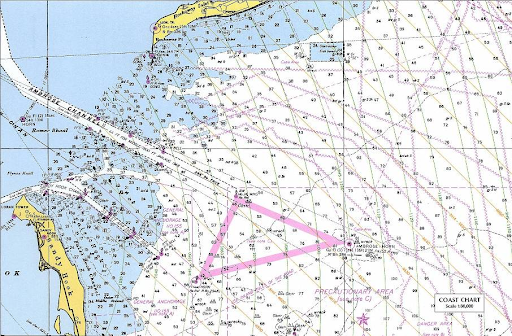
\includegraphics[width=\textwidth]{carteloran}
	\caption{Carte d’une station de base LORAN}
\end{figure}

Le processus de localisation se déroule de la manière suivante : le dispositif mobile calcule la variation de temps entre l'arrivée des signaux de la station maître et d'une station esclave, ce qui génère une ligne de position. Une deuxième ligne de position est obtenue en mesurant une autre variation de temps entre la station principale et une deuxième station secondaire. La convergence de ces deux approches aboutit à la détermination de la position du dispositif mobile \cite{frederic_evennou_techniques_2007}.\\

La navigation s'appuie sur des cartes préétablies. Le récepteur LORAN n'effectue pas de calculs de position par lui-même. Les cartes marines, telles que celle illustrée à la Figure 1.1, représentent les différents décalages observables. L'intersection des diverses ligne de position donne lieu à une approximation de la position du navire. Dans les récepteurs modernes, les valeurs affichées ne sont plus les variations de temps, mais plutôt les coordonnées de latitude et de longitude correspondantes, Les précisions données pour ce système de navigation sont de l’ordre de 500 m. Pour des applications de navigation maritime, cette précision était suffisante avant l’arrivée du GPS \cite{frederic_evennou_techniques_2007}.

\subsubsection{La localisation par réseau GSM}
La localisation par GSM consiste à positionner un terminal GSM en se basant sur des informations liées aux antennes GSM auxquelles le terminal est connecté. La précision de la géolocalisation par GSM varie généralement de 200 mètres à plusieurs kilomètres, en fonction de la localisation du terminal, qu'il soit en milieu urbain ou rural.\\

\noindent Les trois technologies de géolocalisation distinctes utilisées par le GSM sont :

\begin{itemize}
	\item Le différentiel temps dit EOTD (Enhanced Observed Time Difference) : Le téléphone mobile émet un signal vers les stations mobiles environnantes, celle qui est la plus proche lui renvoie ce signal. Le temps écoulé entre l’émission et la réception de cette onde est analysée par un serveur externe qui calculera la localisation du téléphone portable dans le réseau.
	
	\item Le système de l’identification de cellule ou Cell ID (Cellule IDentify) : Le système de l’identification par cellule est la technique de géolocalisation la plus simple et la moins couteuse. Lorsque l’utilisateur se trouve dans une zone couverte par le réseau, il est localisé grâce à l’identification de la cellule à laquelle appartient l’antenne et par laquelle la communication est transmise.
	
	\item La triangulation : Le système de la triangulation repose sur le traitement croisé des informations provenant en permanence de trois relais émetteur et récepteur qui changent au fur et à mesure que l’antenne hertzienne utilisée par le portable de l’usager se déplace.
\end{itemize}

\subsubsection{La géolocalisation par Wi-Fi} 
La géolocalisation par Wi-Fi constitue une solution adaptée tant pour le positionnement à l'intérieur que l'extérieur des bâtiments.
De manière similaire à la méthode Cell ID utilisée pour la géolocalisation sur un réseau GSM, un terminal Wi-Fi peut se localiser en se basant sur les identifiants de bornes Wi-Fi (adresses MAC) qu'il détecte. Des bases de données répertoriant de nombreuses bornes Wi-Fi ainsi que leurs positions géographiques existent. Ces bases de données peuvent être la propriété d'entreprises privées ou être mises à disposition gratuitement par des sociétés.

\subsubsection{Limites des systèmes de localisation par réseaux terrestres }
 
Ces systèmes terrestres possèdent une portée limitée, dans la mesure où ils supposent une surface de localisation plane, ce qui n’est pas le cas de la Terre. De plus, le signal envoyé est affaibli dans l’air, et peut même être dégradé par des obstacles ou par les conditions météorologiques. Malgré tout, ces systèmes sont toujours opérationnels, pour des applications précises comme l’aéronautique, ou en complément des systèmes satellitaires \cite{frederic_evennou_techniques_2007}.

\subsection{ Les systèmes de localisation satellitaires}
L'émergence d'un système mondial de localisation s'est manifestée avec les avancées dans la conquête spatiale dans les années 1960. Les États-Unis ont introduit le tout premier système de positionnement par satellite en 1964, baptisé TRANSIT \cite{w_guier_and_g_weiffenbach_genesis_1997}. Ce système utilisait l'effet Doppler subi par le signal émis, lequel renfermait des informations précises sur la position du satellite émetteur, appelée éphéméride. Cette méthode permettait de se localiser dans le cadre du référentiel géodésique terrestre. Répondant aux exigences militaires, les États-Unis ont entrepris dans les années 1970 le développement d'une solution plus précise. \\

En effet, le système TRANSIT était entravé par les limitations imposées par la propagation du signal satellite dans l'atmosphère, incluant les affaiblissements dus à la troposphère et la dispersion des fréquences dans l'ionosphère. Ces facteurs ne permettaient qu'une précision de l'ordre de quelques centaines de mètres.

\subsubsection{La localisation par GPS}
Le GPS représente le système de localisation le plus répandu parmi les systèmes mondiaux de positionnement par satellites. Il est entièrement opérationnel et accessible partout. En effet, grâce au GPS, il est possible d'obtenir instantanément la localisation précise de n'importe quel endroit sur la planète.

Le système GPS englobe une constellation composée d'au moins 24 satellites tournant autour de la Terre suivant six orbites différentes. Chacune de ces orbites est inclinée à un angle de 55 degrés par rapport à l'équateur terrestre. Les orbites sont réparties de manière à être séparées de 60 degrés les unes des autres, garantissant ainsi une couverture de 260 degrés sur l'ensemble de la planète. Chaque orbite possède un rayon de 26 560 km. Ces orbites sont configurées de manière que les satellites effectuent une révolution complète autour de la Terre en l'espace d'une journée sidérale. Les quatre satellites se trouvant sur une orbite ne se trouvent pas à équidistance sur cette dernière. Deux des satellites sont espacés d'un angle variant entre 30,0 et 32,1 degrés. Les deux autres satellites forment un angle compris entre 92,28 et 130,98 degrés par rapport aux trois autres. Cette configuration a été mise en place afin de minimiser les effets en cas de dysfonctionnement d'un des satellites. Théoriquement, un récepteur GPS devrait être en mesure de capter entre 4 et 11 satellites depuis n'importe quel point de la surface terrestre \cite{frederic_evennou_techniques_2007}.

\subsubsection{GLONASS }
GLONASS est un système russe de navigation par satellite fonctionnant dans le cadre d'un service de radionavigation par satellite. Il constitue une alternative au système de positionnement global et est le deuxième système de navigation en service avec une couverture mondiale et une précision comparable \cite{bernhard_hofmann_wellenhof_gnss}.\\

Le système GLONASS repose sur une constellation de 24 satellites en mouvement, répartis sur 3 plans orbitaux et situés à une altitude de 19 100 km. Le programme GLONASS a été initié en 1982 et a été déclaré opérationnel à part entière en 1993 par les autorités russes. Toutefois, en raison de contraintes financières rencontrées par l'Union Soviétique et de la relativement courte durée de vie des satellites (de 2 à 3 ans), la constellation a progressivement subi une détérioration. À l'heure actuelle, le système fonctionne en mode réduit avec seulement sept satellites opérationnels. Ce système trouve son application en géodésie, grâce à l'utilisation de mesures de phase.\\

L’intérêt de ce système de navigation réside en sa robustesse aux interférences. Chaque satellite émet sur sa propre fréquence (FDMA). Les satellites balaient une plus grande région du globe notamment les regions nord du fait des caractéristiques de la constellation de satellites et du plan d’inclinaison. Le principal défaut du système est qu’il n’est guère entretenu. L’entretien des satellites est très onéreux et du fait que les autorités russes manquent de moyens financiers, aujourd’hui seulement sept satellites sur les vingt quatre sont opérationnels \cite{frederic_evennou_techniques_2007}.

\subsubsection{Galileo}
Galileo est destiné à être un GNSS civil de l'UE qui permet à tous les utilisateurs d'y accéder. À l'origine, le GPS réservait le signal de la plus haute qualité à un usage militaire, et le signal disponible pour un usage civil était intentionnellement dégradé (disponibilité sélective). Cette situation a changé lorsque le président Bill Clinton a signé une directive politique en 1996 pour désactiver la disponibilité sélective. Depuis mai 2000, le même signal de précision est fourni aux civils et aux militaires \cite{bernhard_hofmann_wellenhof_gnss}.\\

Sur le plan conceptuel, GALILEO ne différera pas de manière significative du GPS. Il reposera sur une constellation de 30 satellites, chacun ayant une masse d'environ 700 kg. Ces satellites seront agencés en trois plans orbitaux inclinés à un angle de 56 degrés par rapport à l'équateur, évoluant à une altitude de 23 500 km. Chaque satellite effectuera une rotation complète autour de la Terre en environ 14 heures. La gestion de la constellation sera assurée par un réseau global de stations terrestres \cite{bernhard_hofmann_wellenhof_gnss}.

\section{Localisation d’un terminal par GPS}
Le GPS est un système satellitaire qui est le plus populaire parmi les systèmes de positionnement mondial par satellites qui produit des informations en continu aux récepteurs GPS. Dans la vie quotidienne, les récepteurs GPS sont intégrés à de nombreux objets tels que les téléphones portables, les appareils photo et les automobiles. Ils sont également utilisés dans des dispositifs plus spécialisés tels que les robots d'exploration et les GPS de randonnée.\\

Il est constitué de trois parties distinctes nommées segments qui sont le segment spatial, le segment de contrôle et le segment utilisateur.

\begin{itemize}[label=-]
\item \textit{Le segment spatial}
\end{itemize}


Le segment spatial, composé des satellites, constitue le cœur du système GPS. Ces satellites forment une constellation en orbite autour de la Terre, évoluant à une altitude supérieure à 19 000 km. Cette altitude élevée permet une couverture étendue des signaux sur une large zone. Les orbites des satellites sont organisées de manière à ce qu'à tout moment, un récepteur GPS puisse capter les signaux d'au moins trois satellites simultanément.\\

Les satellites envoient des signaux radio à faible puissance et sur des fréquences différentes. Ces signaux sont capables de traverser des matériaux tels que le plastique, le verre et les nuages, mais ils sont bloqués par des objets denses ou solides tels que les bâtiments et les montagnes. Chaque satellite émet un code unique, ce qui permet aux récepteurs GPS d'identifier et de différencier les signaux émanant de chaque satellite.

\begin{itemize}[label=-]
\item \textit{Le segment de contrôle : }
\end{itemize}

Il assure la supervision des satellites GPS, en les suivant et en leur fournissant des ajustements au niveau du temps et des orbites. Ce segment comprend cinq stations de contrôle réparties dans le monde, chacune étant située à différents endroits autour de la Terre. Parmi ces cinq stations, quatre sont automatisées et sont chargées de la surveillance des satellites, tandis qu'une station principale est dédiée au contrôle global. Les stations automatiques reçoivent des données des satellites et transmettent ces informations à la station de contrôle principale. Cette dernière procède à la mise à jour et à la correction des données reçues, puis renvoie ces informations aux satellites à l'aide de deux antennes situées sur deux autres.

\begin{itemize}[label=-]
	\item \textit{Le segment utilisateur}
\end{itemize}

Le segment utilisateur comprend les utilisateurs militaires et civils qui reçoivent et utilisent les informations émanant des satellites via un récepteur GPS. Ce segment englobe diverses catégories d'utilisateurs, notamment les forces de police, la gendarmerie, les militaires (armée de terre, marine, etc.) dans le domaine militaire. Dans le domaine civil, ce segment rassemble les pilotes, les navigateurs maritimes, les pêcheurs, les sportifs, les chasseurs, les conducteurs d'engins, les randonneurs, et bien d'autres.

\subsection{La trilatération}

Afin de fonctionner correctement, le récepteur GPS doit acquérir deux informations fondamentales : la distance entre lui et les satellites ainsi que les positions exactes de ces satellites. Après avoir capté les signaux émis par les satellites, le récepteur mesure le temps nécessaire à la propagation de ces ondes, ce qui lui permet de calculer la distance qui le sépare de chaque satellite. Cette opération est ensuite répétée pour les autres satellites en vue.
Une fois que les distances entre le récepteur et les satellites sont connues, il devient possible de calculer et de déterminer la position grâce à une technique de triangulation. Pour obtenir une position en deux dimensions, trois satellites sont nécessaires, tandis que pour une position en trois dimensions, quatre satellites sont requis.

\begin{figure}[H]
	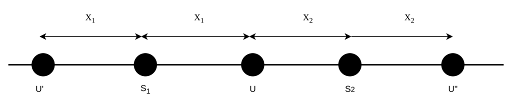
\includegraphics[width=\textwidth]{trilateration1d}
	\caption{Principe du GPS dans un espace 1-D}
\end{figure}

Lorsqu'un équipement U (qu'il s'agisse d'un satellite ou d'un appareil mobile) effectue une mesure et évalue la distance qui le sépare du satellite S1, cela engendre deux positions potentielles pour U : soit à gauche de S1, soit à sa droite. Pour lever cette incertitude de position, l'utilisation d'un second satellite devient nécessaire. Dans ce scénario, c'est le satellite S2 qui intervient pour résoudre cette ambiguïté. Lorsque S2 évalue la distance entre lui et l'équipement U à x2, cela permet de déterminer la seule position plausible, comme illustrée par U sur la figure 1.2.\\

Le processus de détermination de la position d'un équipement dans un espace à deux ou trois dimensions suit une logique similaire à celle utilisée pour la localisation en une dimension. Dans cette configuration, l'obligation est d'avoir trois satellites à partir desquels trois distances sont mesurées. Le lieu géométrique associé à une distance spécifique par rapport à un point fixe est un cercle dans le cas bidimensionnel. La figure 1.3 démontre que deux satellites conduisent à l'estimation de deux positions dans l'espace. Cependant, l'introduction d'un troisième cercle est nécessaire pour déterminer la position unique de l'utilisateur.

\begin{figure}[H]
	\centering
	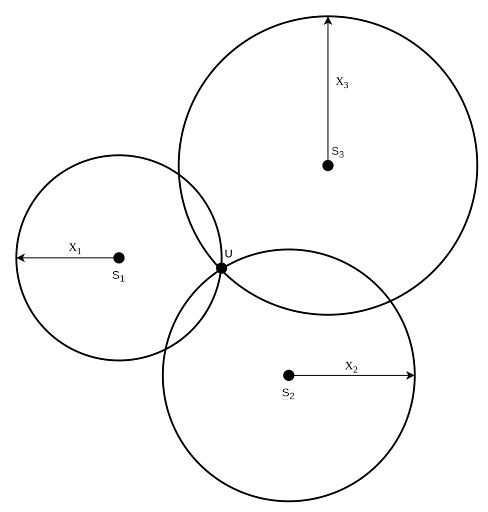
\includegraphics[width=4.48in, height=4.71in]{gps2d}
	\caption{Principe du GPS dans un espace 2-D}
\end{figure}

De la même manière, on aboutit à la nécessité de disposer de quatre satellites pour parvenir à une localisation dans un espace à trois dimensions. Dans cet espace, le lieu géométrique correspondant est une sphère dont le rayon est la distance entre le satellite et l'utilisateur. On sait que l'intersection de deux sphères est un cercle. L'intersection de ce cercle avec une sphère génère deux points dans l'espace, et la troisième sphère détermine quelle position parmi les deux est occupée par l'équipement mobile.

\section{ÉTUDE PRÉALABLE}
Il existe aujourd’hui toute une panoplie des applications utilisant la géolocalisation et pouvant permettre à une personne en danger d’être localisé et de bénéficier d’une assistance. Dans cette partie, nous allons présenter ces applications, ensuite, nous allons établir une étude critique et enfin, nous allons proposer des pistes de solution qui nous permettront d’avoir plus de lumière avant de passer à la conception de notre solution.

\subsection{Étude de l’existant}
\subsubsection{ICE GeoAlert}
\begin{figure}[H]
	\centering
	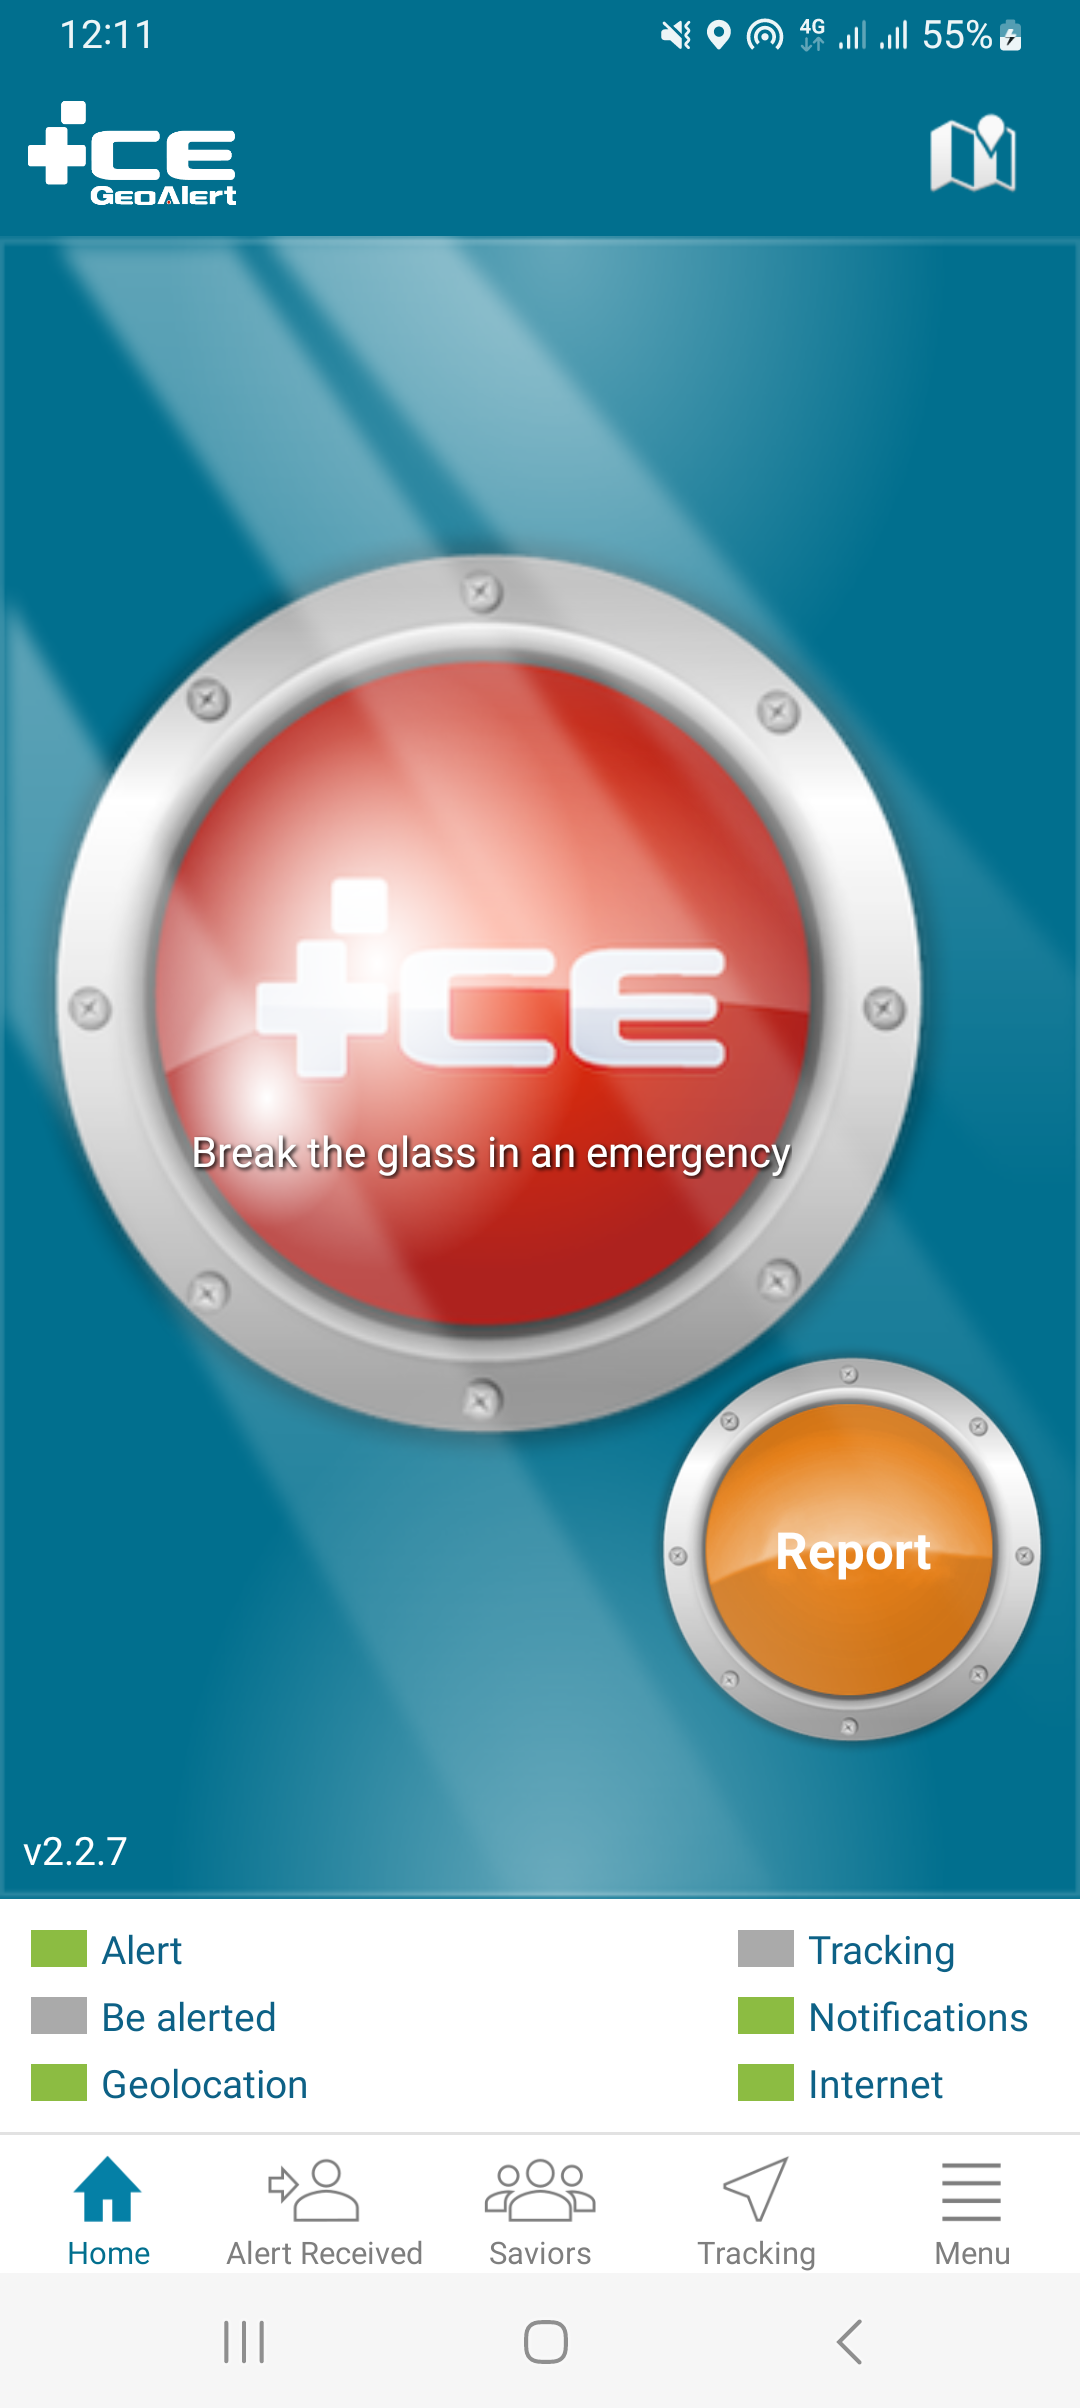
\includegraphics[width=\textwidth]{icegeoalert}
	\caption{Caputre de l’application ICE GeoAlert}
\end{figure}

ICE GeoAlert\footnote{https://icegeoalert.com} est une application qui permet aux utilisateurs d’alerter leurs familles. Pour envoyer un message d’alerte contenant sa géolocalisation à ses proches, la personne en danger doit avoir ICE GeoAlert installé au préalable, et envoie une alerte en cliquant sur le bouton rouge. L’alerte est reçue par message et par email.

\begin{itemize}
	\item Avantages :
	\begin{itemize}
		\item La possibilité d'envoyer rapidement sa géolocalisation aux proches en cas de danger.
		\item Le déclenchement d'une alerte via un bouton dédié, ce qui peut être rapide et intuitif dans une situation d'urgence.
		\item L'alerte est envoyée par message et par e-mail, ce qui garantit que les proches soient informés via plusieurs canaux.
	\end{itemize}
	
	\item Inconvénients :
	\begin{itemize}
		\item Dépendance de la connexion Internet pour envoyer les alertes, ce qui pourrait poser un problème dans des endroits avec une couverture réseau limitée.
		
		\item Nécessité d'une action consciente de la part de la personne en danger pour déclencher l'alerte, ce qui pourrait ne pas être possible dans toutes les situations d'urgence.
	\end{itemize}
	
\end{itemize}

\subsubsection{The Sorority}
\begin{figure}[H]
	\centering
	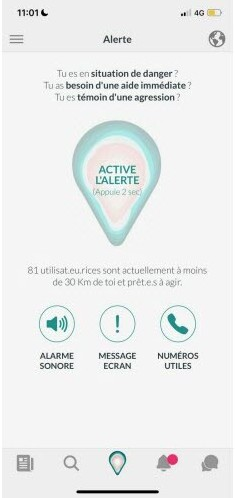
\includegraphics{sorority}
	\caption{Caputre de l’application The Sorority}
\end{figure}

L’application The Sorority\footnote{https://www.jointhesorority.com/} Mise sur l’entraide pour lutter contre le harcèlement de rue en créant une communauté de femmes et personnes issues des minorités de genre, avec des utilisateurs volontaires et aux profils vérifiés.\\ 

En cas de danger, on peut afficher un message en grand sur l’écran de son smartphone pour interpeller directement les personnes autour, déclencher une alarme sonore pour attirer l’attention et dissuader l’agresseur et également appeler les autorités via un raccourci.

Grâce à la géolocalisation, les cinquante utilisateurs les plus proches sont aussi alertés. L’application permet aussi de trouver un lieu sûr où se réfugier en cas de besoin/danger immédiat. L’application aide aussi à lutter contre les violences conjugales, intra-familiales et contre toutes les formes de harcèlement.

\begin{itemize}
	\item Avantages :
	\begin{itemize}
		\item Encouragement à la solidarité et à l'entraide entre utilisatrices pour lutter contre le harcèlement et les agressions.
		\item Fonctionnalités telles que l'affichage de messages d'urgence,le déclenchement d'alarmes sonores et l'appel aux autorités, qui peuvent dissuader les agresseurs.
		\item Géolocalisation pour alerter les utilisateurs proches en cas de danger, ce qui peut permettre une réponse plus rapide.
	\end{itemize}
	
	\item Inconvénients :
	\begin{itemize}
		\item Limitation à un groupe spécifique d'utilisateurs (femmes et minorités de genre), excluant potentiellement d'autres groupes susceptibles d'être en danger.
		
		\item Dépendance de la participation volontaire des utilisateurs, ce qui pourrait réduire la portée de l'application si le nombre d'utilisateurs n'est pas suffisamment élevé.
	\end{itemize}
	
\end{itemize}

\subsection{Critique de l’existant}

Les applications étudiées visent à répondre à des situations d'urgence cruciales, mais elles présentent des défis significatifs. La dépendance à la connectivité Internet peut s'avérer problématique dans les régions où la couverture réseau est limitée. Une autre limitation importante réside dans la nécessité d'une action manuelle de la part de l'utilisateur en danger pour déclencher une alerte. Dans des scénarios de danger extrême, cette action peut être difficile, voire impossible à réaliser, réduisant ainsi l'utilité de ces applications dans des situations critiques.

De plus, les solutions examinées ont des portées limitées. Certaines applications sont restreintes à des groupes spécifiques d'utilisateurs, excluant potentiellement d'autres personnes en danger.
Dans l'environnement spécifique de Lubumbashi, il est impératif de développer des solutions qui surmontent ces limites pour garantir une protection adéquate et une assistance rapide aux individus en danger.

\subsection{Piste de solution}

La conception d'un système d'appel au secours efficace en cas d'enlèvement à Lubumbashi requiert une approche réfléchie et innovante pour surmonter les limites identifiées dans les applications existantes, telles qu'ICE GeoAlert 2014 et The Sorority. Ce chapitre explore diverses pistes de solutions qui pourraient être envisagées pour répondre aux défis spécifiques de la région.

\begin{itemize}
	\item Alertes automatisées par Reconnaissance Sonore : L'intégration d'un système de reconnaissance sonore sur les smartphones des utilisateurs pourrait permettre la détection automatique de signaux de danger, tels que cris ou bruits suspects. Cette fonctionnalité automatisée renforcerait la réactivité du système, déclenchant des alertes sans nécessiter d'action manuelle de la part de l'utilisateur.
	
	\item Envoi d'Alertes par Différents Canaux : Pour assurer que les alertes soient reçues rapidement, il serait bénéfique d'envisager l'envoi d'alertes par différents canaux. Cela inclut non seulement les réseaux mobiles GSM, mais aussi les applications de messagerie instantanée, les courriels et les notifications push.
\end{itemize}

\section{Conclusion partielle}
Dans ce chapitre, les principales méthodes de localisation des utilisateurs mobiles ont été présentées. On distingue les systèmes de localisation par réseaux terrestres tels que le LORAN C, le GSM ou encore le WIFI qui communiquent avec les équipements mobiles par radio. Ces systèmes qui, malgré leurs limites causées par les obstacles et les conditions météorologiques, sont toujours opérationnels, dans des domaines tels que l’aéronautique, ou en complément des systèmes satellitaires. Nous avons également présenté quelques différents systèmes de localisation satellitaire qui sont le GPS, GLONASS et Galileo. Enfin, nous avons présenté le fonctionnement de localisation d’un terminal mobile grâce aux systèmes satellitaire GPS qui est un système compatible avec la majorité des objets de notre vie quotidienne tels que les smartphones et les véhicules automobiles.

	\chapter{CONCEPTION ET MODÉLISATION }
\justifying
\large
\setlength{\parindent}{2.5em}

\section{Introduction Partielle}

Dans ce présent chapitre, nous allons procéder à la réalisation des diagrammes UML qui nous permettront de bien comprendre notre système, en plus des diagrammes, nous allons définir le processus de développement utilisé et du langage utilisé pour dégager lesdits diagrammes.
\subsection{Présentation du langage UML}

UML est un langage de modélisation très complet, qui couvre de nombreux aspects du développement des logiciels, comme les exigences, l’architecture, les structures et les comportements \cite{xavier_blanc_uml2}.
UML est un langage de modélisation visuelle à usage général pour les systèmes. Bien qu'UML soit le plus souvent associé à la modélisation de systèmes logiciels orientés objet, son application est beaucoup plus large que cela \cite{jim_arlow_uml}.
UML n'est pas lié à une méthodologie ou à un cycle de vie spécifique. Il peut d'ailleurs être utilisé avec toutes les méthodologies existantes. La méthode UP par exemple utilise UML comme syntaxe de modélisation visuelle sous-jacente. Elle est la méthode préférée pour UML, car elle est la mieux adaptée, mais UML fournit le support de modélisation visuelle pour d'autres méthodes \cite{jim_arlow_uml}.

\subsection{Présentation de la méthode DSDM}
La méthode DSDM, encore appelée Méthode de développement de systèmes dynamiques, est une méthode de gestion de projet de la catégorie des méthodes agiles développée en Grande-Bretagne à partir de 1994.
La méthode DSDM fait référence à un processus organisé et fondé sur le bon sens qui donne la priorité à la mise en œuvre rapide et efficace de projets.  À bien des égards, elle est comparable à XP et à Scrum, mais son principal avantage par rapport à ces deux méthodes est qu'il s'agit de la meilleure méthodologie pour laquelle les délais sont fixes. Au lieu de se concentrer sur les activités des équipes de développement, DSDM met l'accent sur la livraison de la solution.  Cette méthodologie fait le nécessaire pour s'assurer que le sens commercial et la faisabilité de chaque projet ont été établis avant la conception et la mise en œuvre \cite{jason_bennett_agile}.

\begin{figure}[H]
	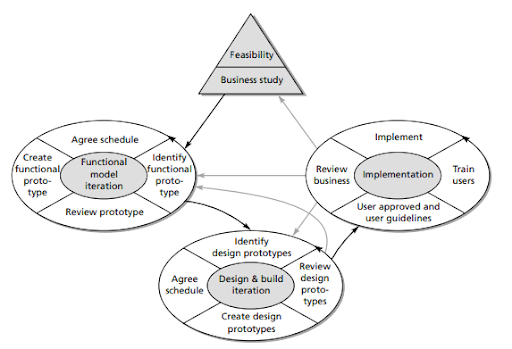
\includegraphics[width=\textwidth]{dsdm}
	\caption{Aperçu général du processus DSDM\cite{the_dsdm_consortium_dsdm}}
\end{figure}


\subsection{Utilisation de l'orienté objet avec le DSDM}
l'analyse orientée objet a commencé par la décomposition du système proposé en cas d'utilisation, qui, pour nos besoins, peuvent être considérés comme des processus métier que le système aidera à résoudre. Cela correspond bien au domaine d'activité de DSDM \cite{the_dsdm_consortium_dsdm}.

\begin{itemize}
	\item Identifier les besoins métier qui devraient être pris en charge par le système proposé.
	\item Définir les besoins en information des processus métier qui seront pris en charge.
	\item Identifier les catégories d'utilisateurs impactés par le développement et l'introduction du système proposé.
	\item Identifier les processus métier et les scénarios métier qui doivent être modifiés.
	\item Clarifier toutes les interfaces avec d'autres systèmes (humains ou automatisés).
	
\end{itemize}

La conception orientée objet consiste essentiellement à sélectionner une architecture (généralement multiniveaux), les protocoles de communication entre les niveaux, une stratégie de gestion au sein des niveaux et les langages appropriés pour construire les niveaux. Encore une fois, cela correspond bien aux objectifs de définition de l'architecture système :

\begin{itemize}
	\item Fournir une compréhension commune des architectures techniques à utiliser pendant le développement et la mise en œuvre.
	\item Décrire la plateforme cible et la plateforme de développement.
	\item Fournir une description générale de l'architecture logicielle (c'est-à-dire les principaux objets ou composants logiciels, à la fois processus et données, et leurs interactions).
\end{itemize}

La technologie orientée objet facilite le développement incrémental du code requis; les concepts d'orientation objet encouragent le développement d'opérations/méthodes de classe petites et réutilisables, qui peuvent être ajoutées au besoin même après que la classe a été déployée \cite{the_dsdm_consortium_dsdm}.


\subsection{Évaluation des risques}
Chaque fonctionnalité d’un logiciel est associée à un risque, qu'il s'agisse d'un risque lié à la disponibilité, à l'évolutivité ou à l'intégrité des données. L'analyse des risques liés à l'architecture est l'une des activités clés de la gestion des projets. En analysant continuellement les risques, l'architecte peut remédier aux lacunes d’un projet et prendre des mesures correctives pour atténuer les risques \cite{mark_richards_fundamentals}.

\section{Besoins}
La conception d’un système exige de connaître les besoins des utilisateurs concernés, voici ci-dessous les besoins que nous avions pu constater; et que nous utiliserons par la suite à des fins de modélisation, enfin de mieux comprendre le système de manière générale.

\subsection{Besoins fonctionnels}
\begin{enumerate}
	\item Les alertes seront envoyées par SMS aux contacts préenregistrés par l'utilisateur ainsi qu'à un tableau de bord géré par un administrateur
	\item L’utilisateur doit s’authentifier avant d’accéder à l’application
	\item L’administrateur doit s’authentifier avant d’accéder à l’espace d’administration
	\item L’utilisateur peut ajouter des contacts qui recevront les alertes
	\item L’utilisateur peut consulter la liste de ses contacts.
	\item L’utilisateur peut modifier les contacts qu’il a ajoutés
	\item L’utilisateur peut supprimer des contacts parmi les contacts qu’il a ajoutés
	\item L'utilisateur peut envoyer des alertes sans manipuler l'écran de son smartphone
	\item L’administrateur peut consulter les alertes émises par les utilisateurs
	\item L'application doit être capable de fonctionner en mode hors ligne.
\end{enumerate}

\subsection{Besoins non fonctionnels}
\begin{enumerate}
	\item l’application doit être intuitive et facile à manipuler
	\item l’application doit être en mesure de fonctionner sur des périphériques non performant 
	\item les informations liées à la géolocalisation des utilisateurs doivent être le plus précises possible
\end{enumerate}

\section{Identification des acteurs}	
\begin{enumerate}
	\item Utilisateur : Une personne qui peut être victime de kidnapping et qui aura besoin d’être assistée
	\item Administrateur : chargé de la gestion du tableau de bord du système
	\item Service de messagerie : un système logiciel externe qui permet d’envoyer des SMS
\end{enumerate}

\section{Diagrammes}
\subsection{Diagramme de cas d’utilisation}
Dans le cadre de notre travail, le diagramme de cas d'utilisation revêt une importance cruciale. Il nous sert avant tout à comprendre les besoins et les exigences fonctionnelles du système que nous analysons ou que nous sommes en train de concevoir. En identifiant les acteurs impliqués et en décrivant comment ils interagissent avec le système, ce diagramme nous permet d'établir une base solide pour la planification et la réalisation de notre solution.

\begin{figure}[H]
	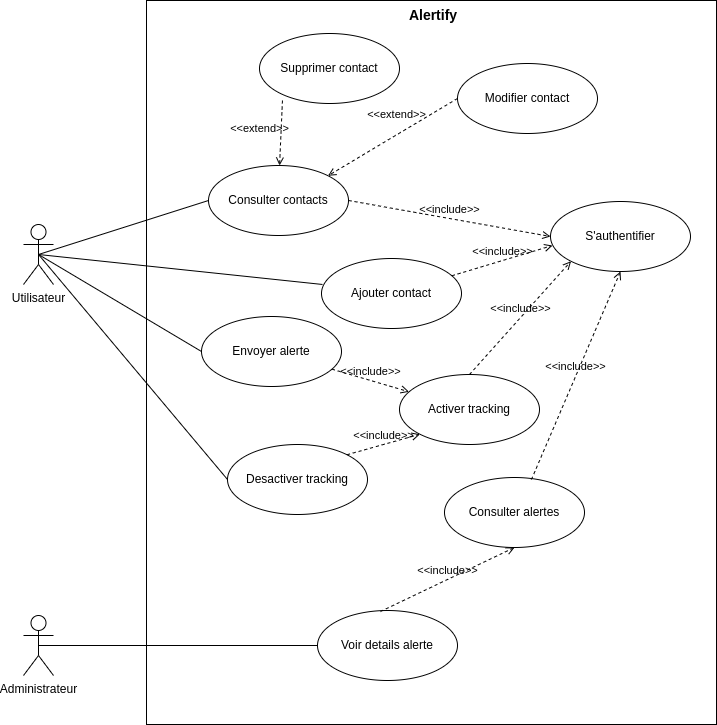
\includegraphics[width=\textwidth]{usecase}
	\caption{Diagramme de cas d’utilisation}
\end{figure}

\subsubsection{Classification des cas d’utilisation}
\begin{table}[H]
	\large
	\captionsetup{justification=raggedright, singlelinecheck=false, font=large,font+=it}
	\caption{Classification des cas d’utilisation}
	\begin{tabularx}{\textwidth}{@{}XXX@{}}
		\hline
		\hline
		\textbf{Cas d’utilisation} & \textbf{Priorité} & \textbf{Risque}\\
		\hline\hline
		S’authentifier & Élevée & Moyen\\
		Consulter contacts & Élevée & Moyen\\
		Ajouter contact & Élevée & Moyen\\
		Modifier contact & Faible & Faible\\
		Supprimer contact & Moyenne & Faible\\
		Activer tracking & Élevée & Moyen\\
		Désactiver tracking & Élevée & Faible\\
		Envoyer alerte & Élevée & Élevée\\
		Consulter alertes & Élevée & Faible\\
		\hline
	\end{tabularx}
\end{table}
\subsubsection{Descriptions textuelles des cas d’utilisation}

\begin{enumerate}[label=\alph*.]
	\item S’authentifier
	\begin{itemize}
		\item Objectif : permettre à l’utilisateur de fournir son identité au système
		\item Acteurs :
		\begin{itemize}
			\item Acteur principal : Utilisateur,Administrateur
			\item Acteur secondaire : -
		\end{itemize}
		\item Précondition : -
		\item Scenario nominal :
		\begin{enumerate}[label=\arabic*.]
			\item L’utilisateur soumet son numéro de téléphone
			\item Le système envoi un code de validation au numéro
			\item Le système affiche le formulaire de soumission du code de confirmation
			\item L’utilisateur soumet le code de confirmation
			\item Le système vérifie la validité du code de confirmation
			\item Le système affiche un formulaire d’insertion d’identité
			\item L’utilisateur soumet son identité
			\item Le système affiche un message de succès 
		\end{enumerate}
		\item Scenario alternatif :
		\begin{enumerate}[label=\arabic*.]
		\item[6] .a. Le code de confirmation est invalide
		\item[6] .a.1. Le système affiche un message d’erreur
		\item[6] .a.2. On rentre au scenario 1
		\end{enumerate}
		\item Scenario d’exception : 
		\begin{enumerate}[label=\arabic*.]
			\item L’utilisateur quitte l’application avant la fin de l’authentification
		\end{enumerate}
		\item Postcondition : L’utilisateur est authentifié et peut accéder aux autres fonctionnalités
	\end{itemize}
	
	\item Consulter contacts
	\begin{itemize}
		\item Objectif : permettre à l’acteur de voir la liste de ses contacts
		\item Acteurs :
		\begin{itemize}
			\item Acteur principal : Utilisateur
			\item Acteur secondaire : -
		\end{itemize}
		\item Précondition : S’authentifier
		\item Scenario nominal :
		\begin{enumerate}[label=\arabic*.]
			\item L’acteur accède à la page des contacts
			\item Le programme affiche la liste de tous ses contacts
		\end{enumerate}
		\item Scenario alternatif : -
	
		\item Scenario d’exception :  -
		\item Postcondition : -
	\end{itemize}
	
	\item Ajouter contact
	\begin{itemize}
		\item Objectif : permettre à l’acteur d’ajouter un contact
		\item Acteurs :
		\begin{itemize}
			\item Acteur principal : Utilisateur
			\item Acteur secondaire : -
		\end{itemize}
		\item Précondition : -
		\item Scenario nominal :
		\begin{enumerate}[label=\arabic*.]
			\item L’utilisateur accède à la page d’ajout de contact
			\item Le formulaire d’ajout est affiché
			\item L’utilisateur soumet le formulaire
			\item Le système vérifie que les informations sont valides
			\item Le système enregistre le contact
			\item Le système affiche un message de succès
		\end{enumerate}
		\item Scenario alternatif :
		\begin{enumerate}[label=\arabic*.]
			\item[5] .a. Les informations sont invalides
			\item[5] .a.1. Le système affiche un message d’erreur
			\item[5] .a.2. On rentre au scenario 2
		\end{enumerate}
		\item Scenario d’exception : -
		\item Postcondition : Un nouveau contact est ajouté
	\end{itemize}
	
	\item Modifier contact
	\begin{itemize}
		\item Objectif : permettre à l’utilisateur de modifier un contact
		\item Acteurs :
		\begin{itemize}
			\item Acteur principal : Utilisateur
			\item Acteur secondaire : -
		\end{itemize}
		\item Précondition : Consulter contact
		\item Scenario nominal :
		\begin{enumerate}[label=\arabic*.]
			\item L’utilisateur sélectionne un contact
			\item L’utilisateur sélectionne l’option de modification du contact
			\item Le système affiche le formulaire de modification du contact
			\item L’utilisateur modifie le contact
			\item L’utilisateur soumet le formulaire
			\item Le système vérifie les nouvelles informations
			\item Le système enregistre les modifications du contact
			\item Le système affiche un message de succès
		\end{enumerate}
		\item Scenario alternatif :
		\begin{enumerate}[label=\arabic*.]
			\item[7] .a. Les informations sont invalides
			\item[7] .a.1. Le système affiche un message d’erreur
			\item[7] .a.2. On rentre au scenario 3
		\end{enumerate}
		\item Scenario d’exception : 
		\begin{enumerate}[label=\arabic*.]
			\item L’utilisateur n’a aucun contact
			\item L’utilisateur quitte la page de modification du contact avant de l’avoir soumis
		\end{enumerate}
		\item Postcondition : Un contact a été modifié
	\end{itemize}	
	
	\item Supprimer contact
	\begin{itemize}
		\item Objectif : permettre à l’utilisateur de supprimer un contact
		\item Acteurs :
		\begin{itemize}
			\item Acteur principal : Utilisateur
			\item Acteur secondaire : -
		\end{itemize}
		\item Précondition : Consulter contact
		\item Scenario nominal :
		\begin{enumerate}[label=\arabic*.]
			\item L’utilisateur sélectionne un contact
			\item L’utilisateur sélectionne l’option de suppression
			\item Le système demande à l’utilisateur de confirmer la suppression
			\item L’utilisateur confirme la suppression
			\item Le contact est supprimé
			\item Le système affiche un message de succès
		\end{enumerate}
		\item Scenario alternatif :
		\begin{enumerate}[label=\arabic*.]
			\item[4] .a. L’utilisateur annule la suppression
			\item[4] .a.1. Le système affiche la liste des contacts
		\end{enumerate}
		\item Scenario d’exception : 
		\begin{enumerate}[label=\arabic*.]
			\item L’utilisateur n’a aucun contact
		\end{enumerate}
		\item Postcondition : Un contact a été supprimé
	\end{itemize}
	
	\item Activer tracking
	\begin{itemize}
		\item Objectif : permettre à l’utilisateur d’activer l’écoute de la commande vocale
		\item Acteurs :
		\begin{itemize}
			\item Acteur principal : Utilisateur
			\item Acteur secondaire : -
		\end{itemize}
		\item Précondition : S’authentifier
		\item Scenario nominal :
		\begin{enumerate}[label=\arabic*.]
			\item L’utilisateur clique sur l’option d’activation de tracking
		\end{enumerate}
		\item Scenario alternatif : -
		\item Scenario d’exception : -
		\item Postcondition : Le système est en attente d’une commande vocale
	\end{itemize}
	
	\item Désactiver tracking
	\begin{itemize}
		\item Objectif : permettre à l’acteur d’annuler l’écoute de la commande vocale
		\item Acteurs :
		\begin{itemize}
			\item Acteur principal : Utilisateur
			\item Acteur secondaire : -
		\end{itemize}
		\item Précondition : Activer tracking
		\item Scenario nominal :
		\begin{enumerate}[label=\arabic*.]
			\item L’utilisateur clique sur l’option de désactivation du tracking
		\end{enumerate}
		\item Scenario alternatif : -
		\item Scenario d’exception : -
		\item Postcondition : L’écoute de la commande vocale est désactivée
	\end{itemize}
	
	\item Envoyer alerte
	\begin{itemize}
		\item Objectif : permettre à l’utilisateur d’envoyer une alerte à ses contacts
		\item Acteurs :
		\begin{itemize}
			\item Acteur principal : Utilisateur
		\end{itemize}
		\item Précondition : Activer tracking
		\item Scenario nominal :
		\begin{enumerate}[label=\arabic*.]
			\item L’utilisateur énonce une commande vocale
			\item Le système vérifie la validité de la commande
			\item Tant que le tracking est active, Le service de messagerie envoie une alerte aux contacts de l’utilisateur
		\end{enumerate}
		\item Scenario alternatif :
		\begin{enumerate}[label=\arabic*.]
			\item[1] .a. Le système détecte un son suspect
			\item[1] .a.1. On passe au scenario 3
			\item[1] .b. L'utilisateur appuie sur le button d'envois d'une alerte
			\item[1] .b.1. On passe au scenario 3
		\end{enumerate}
		\item Scenario d’exception : 
		\begin{enumerate}[label=\arabic*.]
			\item Le Service de messagerie ne fonctionne pas
			\item Fausse alerte
		\end{enumerate}
		\item Postcondition : Alertes envoyées avec succès
	\end{itemize}
	
	\item Consulter alertes
	\begin{itemize}
		\item Objectif : permettre à l’administrateur de voir les alertes envoyées par les utilisateurs
		\item Acteurs :
		\begin{itemize}
			\item Acteur principal : Administrateur
			\item Acteur secondaire : -
		\end{itemize}
		\item Précondition : S’authentifier
		\item Scenario nominal :
		\begin{enumerate}[label=\arabic*.]
			\item L’administrateur demande la page des alertes
			\item Le système affiche la liste de toutes les alertes
		\end{enumerate}
		\item Scenario alternatif : -
		\item Scenario d’exception : -
		\item Postcondition : -
	\end{itemize}
		
	\item Voir détails alerte
	\begin{itemize}
		\item Objectif : permettre à l’administrateur de voir les détails d’une alerte envoyée par les utilisateurs
		\item Acteurs :
		\begin{itemize}
			\item Acteur principal : Administrateur
			\item Acteur secondaire : -
		\end{itemize}
		\item Précondition : Consulter alertes
		\item Scenario nominal :
		\begin{enumerate}[label=\arabic*.]
			\item L’administrateur demande la page des détails d’une alerte
			\item Le système affiche les détails de l’alerte
		\end{enumerate}
		\item Scenario alternatif : -
		\item Scenario d’exception : -
		\item Postcondition : -
	\end{itemize}
\end{enumerate}

\subsection{Diagrammes de séquence}

Dans le cadre de notre travail, le diagramme de séquence nous permet de modéliser les interactions entre les objets ou composants du système, en mettant en évidence la séquence des messages échangés au fil du temps. Ce diagramme est essentiel pour comprendre le comportement dynamique du système, ce qui facilite la conception ainsi que le développement.

\subsubsection{S'authentifier}
\begin{figure}[H]
	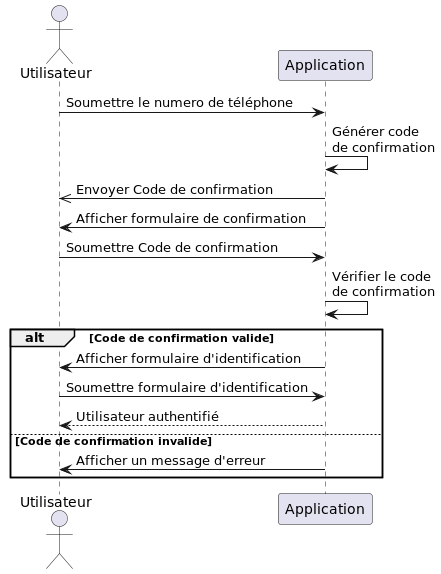
\includegraphics[width=300px]{s_authentifier}
	\caption{Diagramme de séquence S’authentifier}
\end{figure}

\subsubsection{Consulter contacts}
\begin{figure}[H]
	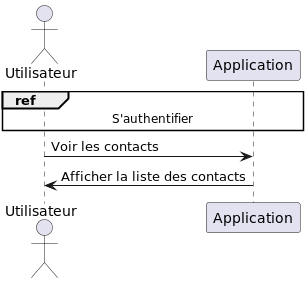
\includegraphics[width=200px]{consulter_contacts}
	\caption{Diagramme de séquence Consulter contacts}
\end{figure}

\subsubsection{Ajouter contact}
\begin{figure}[H]
	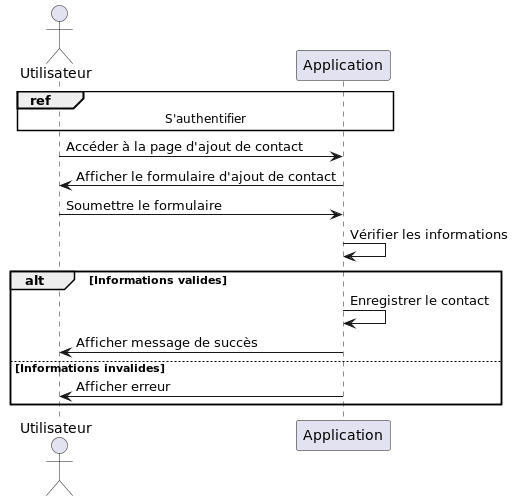
\includegraphics[width=300px]{ajouter_contact.png}
	\caption{Diagramme de séquence Ajouter contact}
\end{figure}

\subsubsection{Supprimer contact}
\begin{figure}[H]
	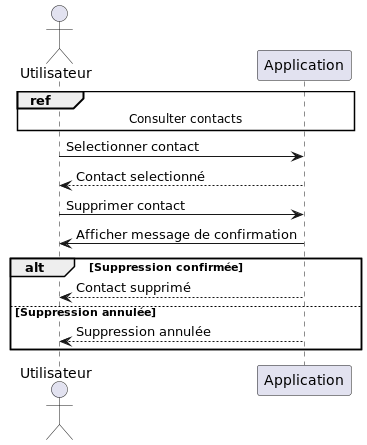
\includegraphics[width=250px]{supprimer_contact}
	\caption{Diagramme de séquence Supprimer contact}
\end{figure}

\subsubsection{Modifier contact}
\begin{figure}[H]
	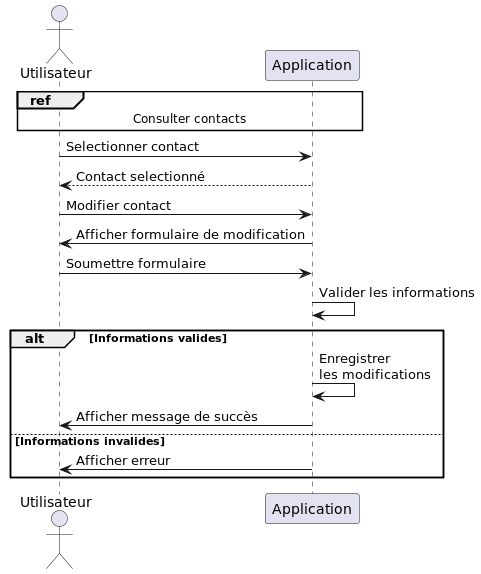
\includegraphics[width=300px]{modifier_contact.png}
	\caption{Diagramme de séquence Modifier contact}
\end{figure}

\subsubsection{Activer tracking}
\begin{figure}[H]
	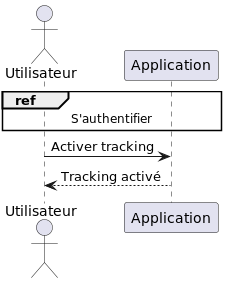
\includegraphics[width=180px]{activer_tracking}
	\caption{Diagramme de séquence Activer tracking}
\end{figure}

\subsubsection{Désactiver tracking}
\begin{figure}[H]
	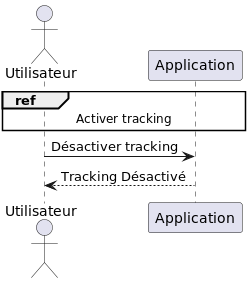
\includegraphics[width=180px]{desactiver_tracking}
	\caption{Diagramme de séquence Désactiver tracking}
\end{figure}

\subsubsection{Envoyer alerte}
\begin{figure}[H]
	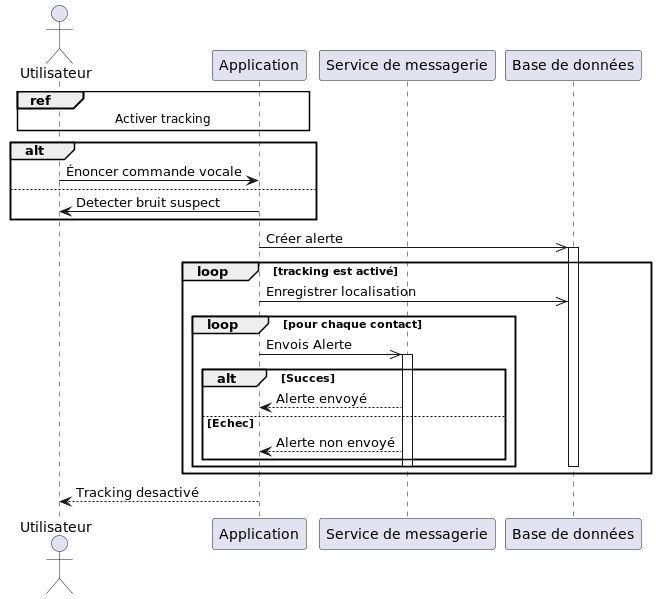
\includegraphics[width=\textwidth]{envoyer_alerte}
	\caption{Diagramme de séquence Envoyer alerte}
\end{figure}

\subsubsection{Consulter alertes}
\begin{figure}[H]
	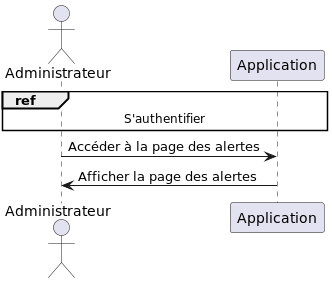
\includegraphics[width=240px]{consulter_alertes}
	\caption{Diagramme de séquence Consulter alertes}
\end{figure}

\subsubsection{Voir détails alertes}
\begin{figure}[H]
	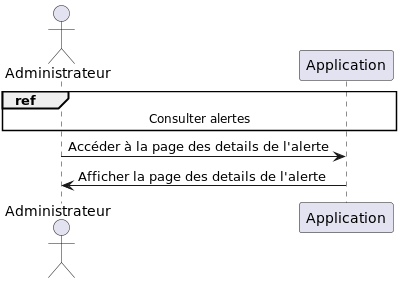
\includegraphics[width=260px]{voir_details_alerte}
	\caption{Diagramme de séquence Voir détails alertes}
\end{figure}

\subsection{Diagramme d’activité}
le diagramme d'activité quant à lui nous permet de modéliser visuellement les processus, les flux de travail, et les décisions au sein du système. En utilisant ce diagramme, nous pouvons mieux comprendre et représenter les séquences d'actions, les transitions, et les conditions qui gouvernent le comportement du système. Cela facilite la planification, la conception et l'optimisation des processus.

\subsubsection{Activité utilisateur}
\begin{figure}[H]
	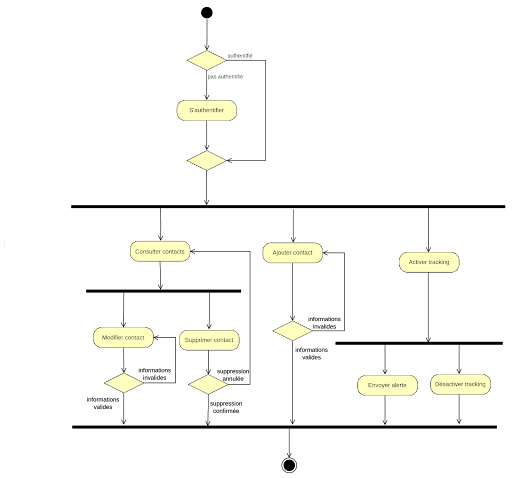
\includegraphics[width=\textwidth]{activity_user}
	\caption{Diagramme d’activité utilisateur}
\end{figure}

\subsubsection{Activité administrateur}
\begin{figure}[H]
	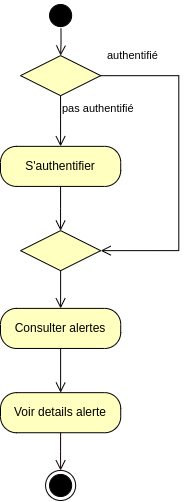
\includegraphics[height=400px]{activity_admin}
	\caption{Diagramme d’activité administrateur}
\end{figure}

\subsection{Modèle de domaine}
\begin{figure}[H]
	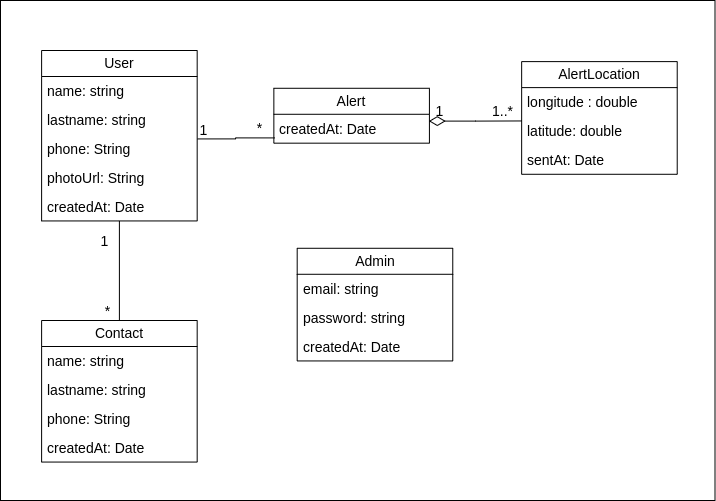
\includegraphics[width=\textwidth]{domain}
	\caption{Modèle de domaine}
\end{figure}

\section{Modélisation de la base de donnes NoSQL orientée document}
La modélisation de la base de données NoSQL constitue une étape cruciale de l'implémentation de notre système. Nous avons opté d’utiliser le service firestore qui propose une base de donnes non relationnelle, sa capacité à gérer efficacement des données géospatiales, sa prise en charge de la synchronisation en temps réel, ainsi que sa scalabilité, en font un choix idéal pour notre application qui nécessite une réactivité immédiate en cas d'urgence.\\

Contrairement aux bases de données relationnelles traditionnelles qui ont une forme simple de disposition en lignes et en colonnes. Une base de données orientée documents stocke les informations au format texte, qui consiste en des collections d'enregistrements organisés selon le concept clé-valeur, c'est-à-dire que pour chaque valeur représentée, un nom (ou étiquette) est attribué, qui décrit sa signification. Ce  modèle de stockage est connu sous le nom d'objet JSON.

\subsection{Règles de mappage pour une base de donnée orientée document}
\subsubsection{Relation par référence}
Ce type de relation stocke les données en incluant des liens ou des références, d'un document à l'autre. Les applications peuvent résoudre ces références pour accéder aux données connexes dans la structure du document lui-même \cite{harley_vera_data}.
\subsubsection{Documents imbriqués}
Ce type de relation est stocké dans une structure de document unique, où les documents imbriqués sont disposés dans un champ ou un tableau. Ces modèles de données dénormalisées permettent de manipuler les données en une seule transaction \cite{harley_vera_data}.

\subsection{Modèle non relationnel}
Voici la manière dont nous avons organisé nos donnes, en priorisant la réduction du nombre de requêtes lors de la lecture.

\begin{figure}[H]
	\centering
	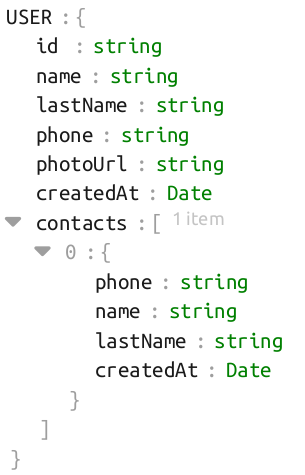
\includegraphics[width=2.23in, height=3.461in,frame]{doc_user}
	\caption{Document utilisateur contenant des sous-documents Contact}
\end{figure}

\begin{figure}[H]
	\centering
	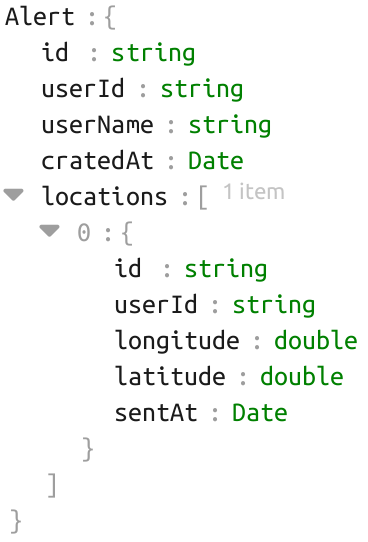
\includegraphics[width=2.23in, height=3.461in,frame]{doc_alert}
	\caption{Document Alert contenant des sous-documents AlertLocation}
\end{figure}

\section{Conclusion partielle}
Pour chaque système d'information, une étape essentielle consiste à le modéliser pour orienter sa concrétisation. Le but de ce chapitre était d'expliquer en détail le fonctionnement du système en utilisant des diagrammes UML. Nous aspirons à atteindre notre objectif, car l'utilisation de multiples diagrammes UML nous a offert une variété de perspectives qui nous seront utiles dans la partie suivante de notre travail, qui sera dédiée à la mise en place de notre solution.


	\chapter{PROCESSUS ET IMPLÉMENTATION}
\justifying
\large
\setlength{\parindent}{2.5em}

\section{Introduction}
Nous en sommes au dernier chapitre de notre travail, ce chapitre se concentrera sur la mise en œuvre de notre solution. Il aura pour mission de mettre en évidence toute la partie technique de notre système. Nous dévoilerons également les défis rencontrés en cours de route, ainsi que les solutions que nous avons adoptées afin de les surmonter. Ce chapitre marque le point culminant de nos efforts pour créer un système d'appel au secours efficace et centré sur l'expérience utilisateur.

\section{Présentation de l'architecture physique}
Une architecture est appelée architecture physique, parfois aussi architecture technique quand elle décrit la façon dont les composants matériels du système communiquent entre eux, ces éléments peuvent être : 

\begin{itemize}
	\item Le poste de travail
	\item Matériel de stockage
	\item Équipement de réseau
	\item Etc…
\end{itemize}

Dans le cadre de notre application, nous avons opté pour une architecture serverless, un élément clé à noter est que la logique métier de l'application réside au sein des clients eux-mêmes. Contrairement à une architecture traditionnelle où la logique métier est souvent centralisée sur un serveur distant, notre approche décentralisée permet aux clients d'exécuter localement la logique métier. 

Cette conception distribuée permet une plus grande réactivité de l'application, réduisant ainsi les dépendances vis-à-vis du serveur distant. Firebase, quant à lui, joue un rôle essentiel en fournissant les services nécessaires pour stocker et synchroniser les données, gérer l'authentification des utilisateurs et faciliter la communication entre les clients et les services cloud. Ainsi, Firebase agit comme une infrastructure backend sans héberger directement la logique métier, offrant ainsi une solution serverless robuste pour notre application.

\begin{figure}[H]
	\centering
	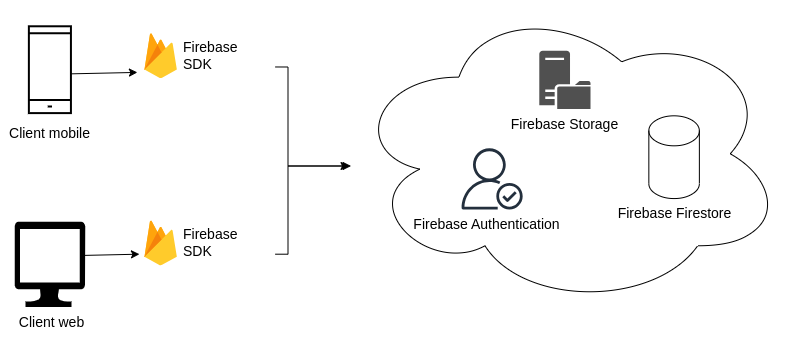
\includegraphics[width=\textwidth]{architecture}
	\caption{Présentation de l'architecture physique}
\end{figure}

\section{Technologies utilisées}
\subsection{Kotlin}
Kotlin est un langage de programmation orienté objet, à typage statique, interopérable avec la machine virtuelle Java, les bibliothèques de classes Java et Android.
Il peut être utilisé presque partout où Java est utilisé, pour le développement côté serveur, les applications Android et bien plus encore. Kotlin fonctionne parfaitement avec toutes les et s'exécute avec le même niveau de performance que Java \cite{dmitry_jemerov_kotlin}.

\subsection{TensorFlow lite}
TensorFlow Lite est une version légère du framework TensorFlow, spécialement conçue pour exécuter des modèles d'apprentissage automatique sur des appareils mobiles et des systèmes embarqués. Son principal avantage réside dans sa capacité à maintenir des performances élevées tout en étant optimisé pour des environnements aux ressources limitées. TensorFlow Lite  permet de déployer des modèles d'intelligence artificielle directement sur des smartphones, des objets connectés, et même des microcontrôleurs, ouvrant ainsi la porte à une gamme étendue d'applications, de la vision par ordinateur à la reconnaissance vocale, le tout en conservant une faible empreinte mémoire et une exécution rapide \cite{ml_2023}.

\subsection{Mediapipe}
MediaPipe est un outil développé par Google qui offre des outils et des modèles pour le traitement des médias en temps réel, y compris la vision par ordinateur et le suivi de mouvement. Il simplifie le déploiement des modèles de machine learning sur des périphériques tels que des smartphones avec des bibliothèques low code. Ces bibliothèques comprennent actuellement des outils pour trois catégories : la vidéo, l'audio et le texte.

\subsection{Yamnet}
YAMNet\cite{yamnet} est un réseau neuronal préformé qui utilise l'architecture de convolution séparable en profondeur MobileNetV1 \cite{andrew_g_howard_menglong_zhu_bo_chen_dmitry_kalenichenko_weijun_wang_tobias_weyand_marco_andreetto_hartwig_adam_mobilenets}. Il peut utiliser une forme d'onde audio comme entrée et faire des prédictions indépendantes pour chacun des 521 événements audio du corpus AudioSet \cite{dataset_large_scale}.

\subsection{Firebase}
Firebase est une plateforme de développement d'applications mobiles et web appartenant à Google, qui offre un ensemble de services cloud, tels que des bases de données en temps réel, l'authentification des utilisateurs, l'hébergement web, le stockage de fichiers, et des outils d'analyse avancés. Elle simplifie considérablement le développement d'applications en fournissant des fonctionnalités prêtes à l'emploi, ce qui permet aux développeurs de se concentrer sur la création de fonctionnalités uniques tout en bénéficiant de la puissance du cloud pour la gestion des données et des utilisateurs.

\subsection{Angular}
Angular est un framework de développement d'applications web open-source développé par Google. Il est largement utilisé pour la création d'applications web modernes et dynamiques. Angular est basé sur le langage TypeScript, une version améliorée de JavaScript, et offre un ensemble complet de fonctionnalités pour simplifier le développement front-end. 

\subsection{Android Studio}
Android Studio est un environnement de développement intégré officiellement pris en charge par Google pour la création d'applications Android. Il offre aux développeurs un ensemble complet d'outils pour concevoir, développer, déboguer et déployer des applications Android. 

\section{Diagramme de déploiement}
\begin{figure}[H]
	\centering
	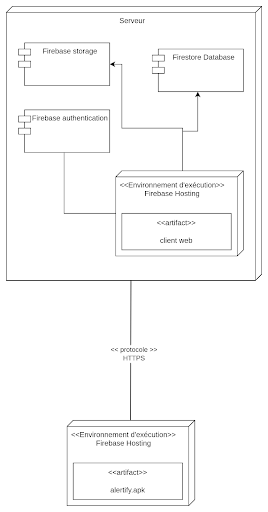
\includegraphics{deploiement}
	\caption{Diagramme de déploiement}
\end{figure}

\section{Expérience utilisateur et fonctionnement}
\subsection{Expérience utilisateur}
Le processus de conception de l'expérience utilisateur consiste à s'assurer qu'aucun aspect de l'expérience de l'utilisateur avec une solution ne se produit sans l’intention consciente et explicite de ce dernier. Cela signifie qu'il faut prendre en compte chaque possibilité de chaque action que l'utilisateur est susceptible de faire et de comprendre ses attentes à chaque étape du processus \cite{jesse_james_garrett_elements}.\\

Dans le cadre de notre travail, l'attention portée à l'UX est cruciale pour garantir l'adoption et l'efficacité du système par les utilisateurs finaux.

Tout d'abord, il est essentiel de comprendre les besoins, les compétences techniques et les préférences des utilisateurs potentiels à Lubumbashi. Cette compréhension approfondie permettra de concevoir une interface utilisateur conviviale et intuitive, adaptée au contexte local. Il est crucial que l'application soit facile à comprendre et à utiliser, même pour les utilisateurs peu familiers avec les technologies modernes.

\subsection{Fonctionnement}

Pour permettre à notre application mobile de recevoir des commandes, nous avons recouru au composant d’application appelé service. Un service est un composant d'application qui peut effectuer des opérations de longue durée en arrière-plan. Il ne fournit pas d'interface utilisateur. Une fois lancé, un service peut continuer à fonctionner pendant un certain temps, même après que l'utilisateur a basculé vers une autre application \cite{services}. Mais avant tout, nous devrions commencer par demander la permission d'accéder à la géolocalisation ainsi qu'au périphérique audio du smartphone, notamment le microphone.

Une fois que l'application a obtenu l'accès au microphone, les données captées sont évaluées à l'aide de MediaPipe et TensorFlow Lite. MediaPipe et TensorFlow Lite ont respectivement pour objectif de détecter des bruits tels que les pleurs et les gémissements, qui peuvent indiquer qu'une personne est en danger, ainsi que des commandes vocales spécifiques. Ces scénarios déclenchent alors le lancement d'alertes. Les alertes entraînent l'envoi de messages contenant la géolocalisation du smartphone aux contacts préenregistrés, ainsi qu'au serveur backend, dans le cas où le smartphone dispose d'une connexion Internet.

\begin{figure}[H]
	\centering
	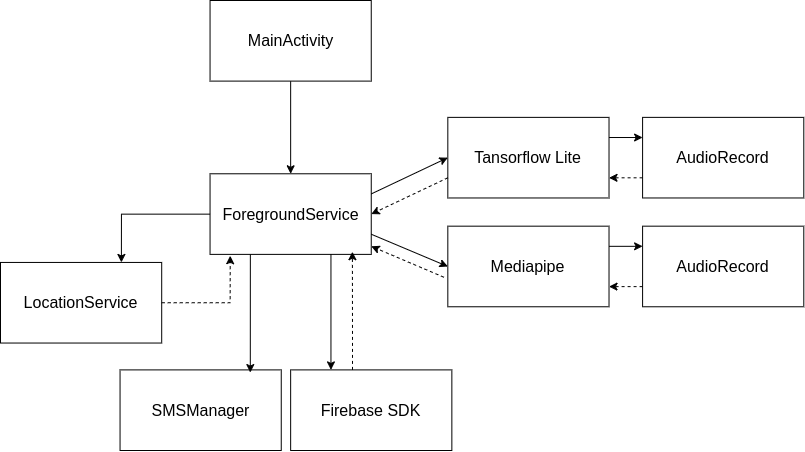
\includegraphics[width=\textwidth]{fonctionnement}
	\caption{Communication des différentes composantes lors de l’envoi d’une alerte}
\end{figure}

\begin{figure}[H]
	\centering
	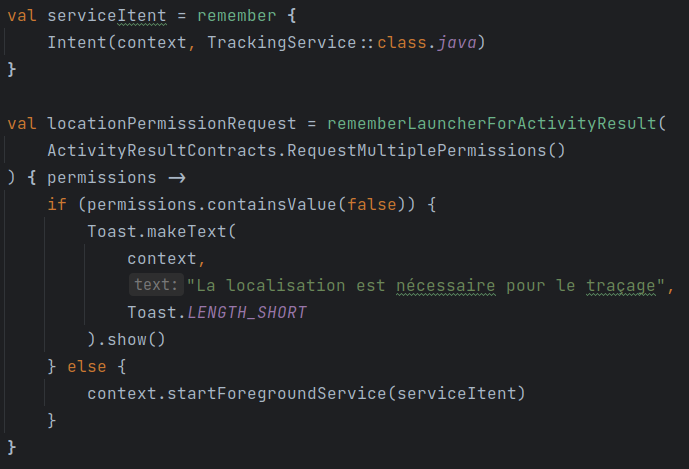
\includegraphics[width=\textwidth]{code_permission}
	\caption{Demande de permission et lancement du service TrackingService}
\end{figure}

\begin{figure}[H]
	\centering
	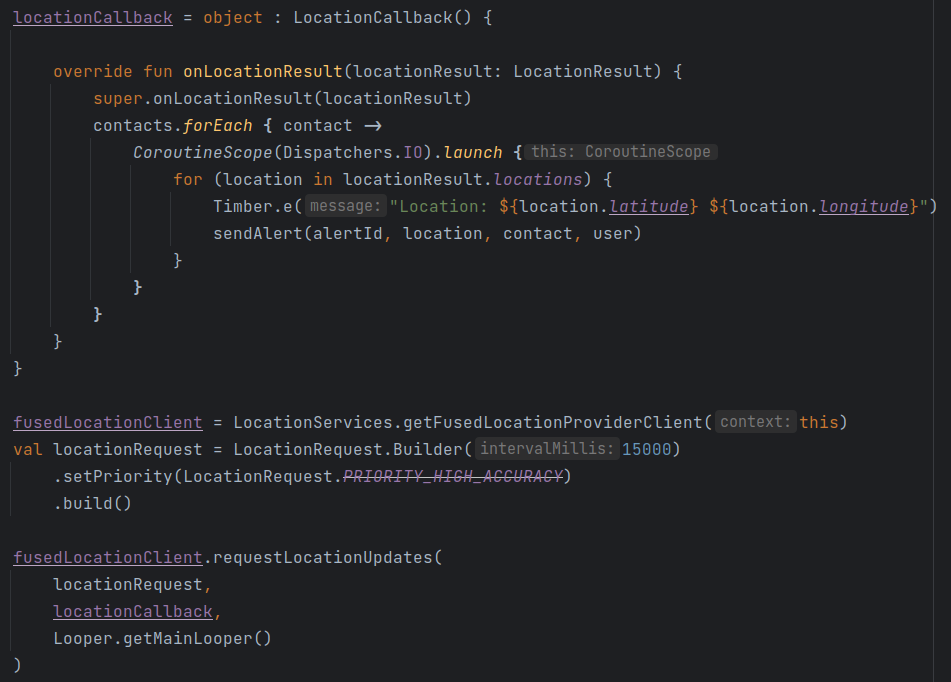
\includegraphics[width=\textwidth]{code_location}
	\caption{Récupération de la localisation}
\end{figure}

\begin{figure}[H]
	\centering
	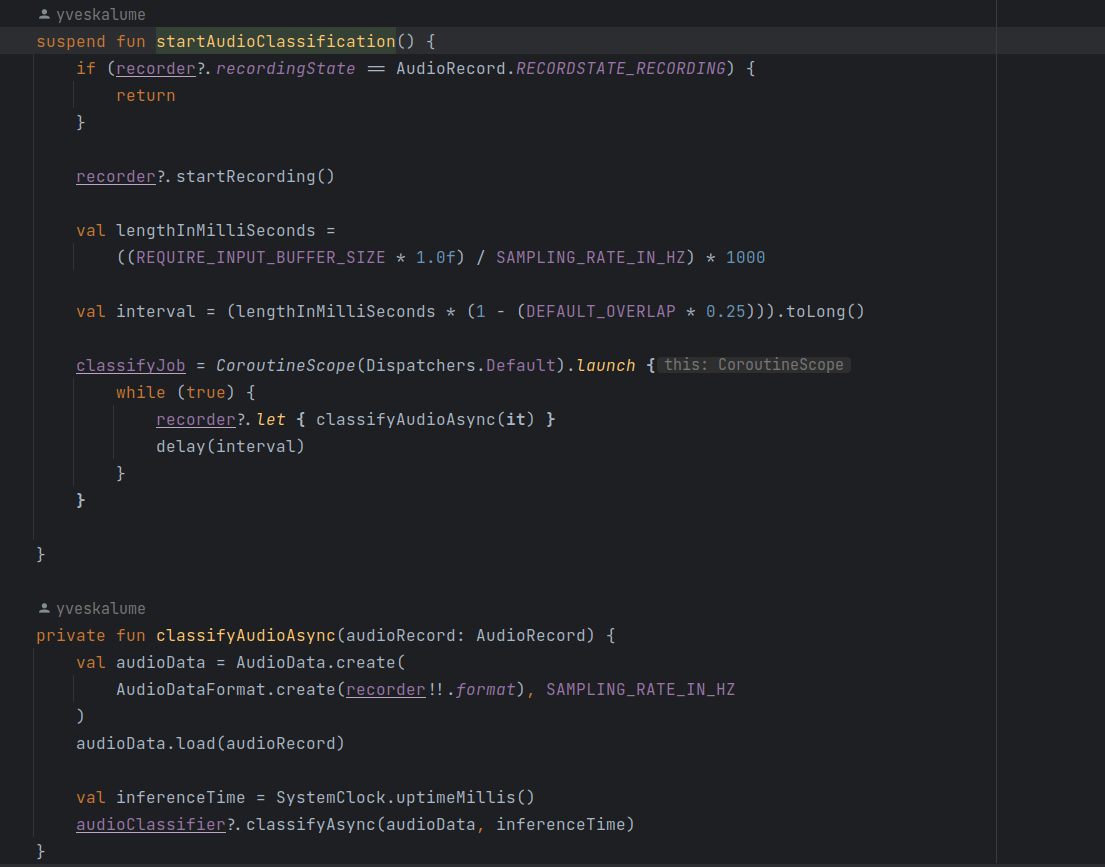
\includegraphics[width=\textwidth]{code_classification}
	\caption{Classification des entrées sonores}
\end{figure}

\begin{figure}[H]
	\centering
	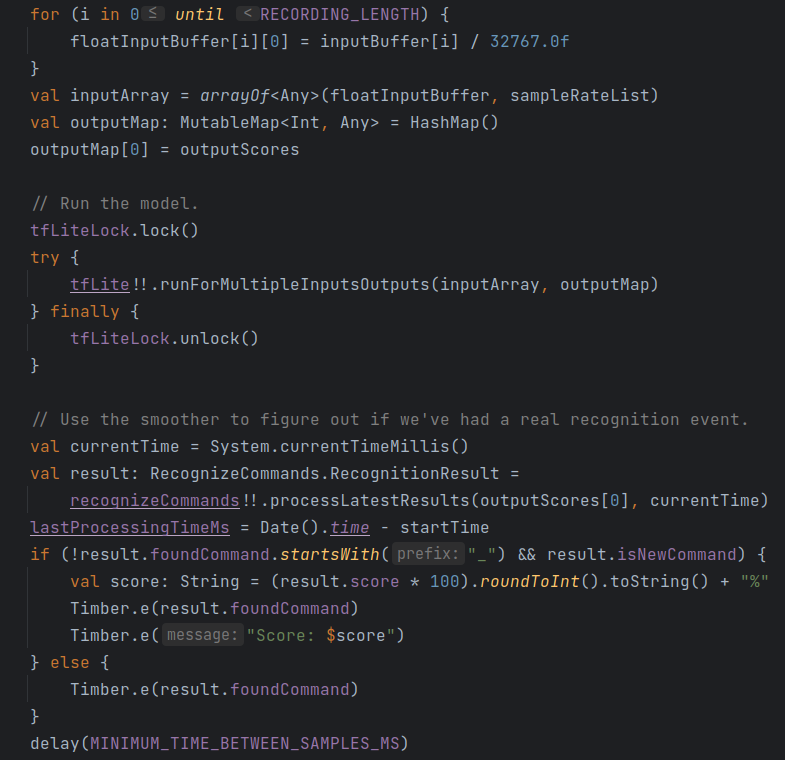
\includegraphics[width=\textwidth]{code_detection}
	\caption{Détection d’une commande vocale sur les entrées audios}
\end{figure}

\begin{figure}[H]
	\centering
	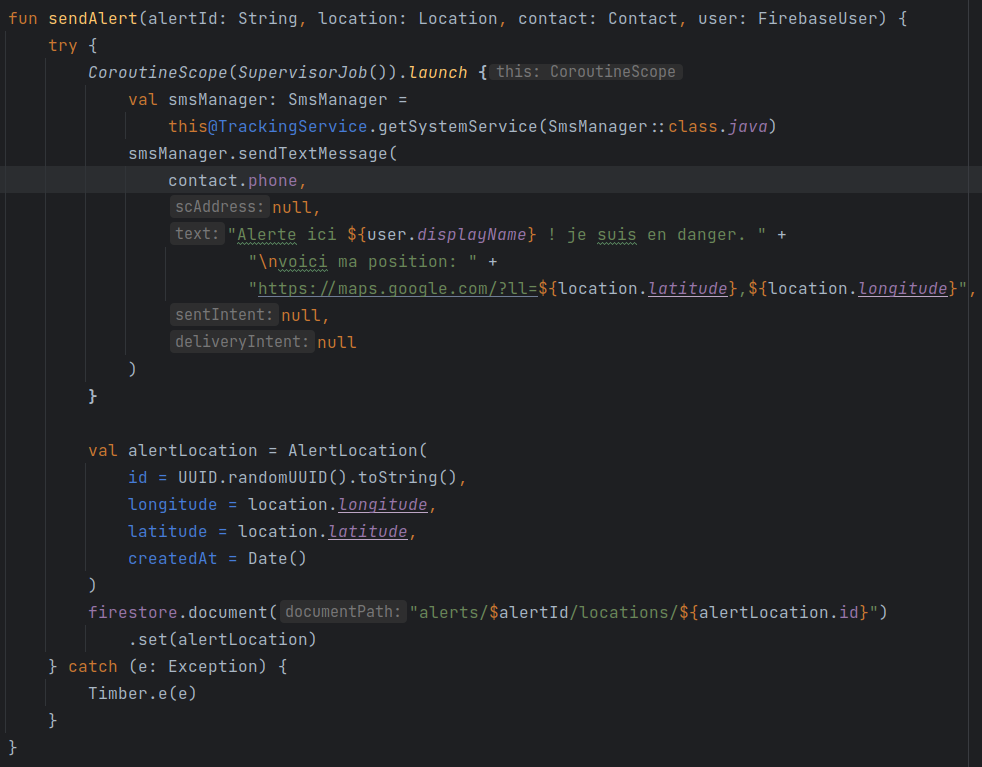
\includegraphics[width=\textwidth]{code_envoi_alerte}
	\caption{Envois d’alertes}
\end{figure}

\section{Captures d’écrans}
\subsection{Client mobile pour utilisateur}

\begin{figure}[H]
	\centering
	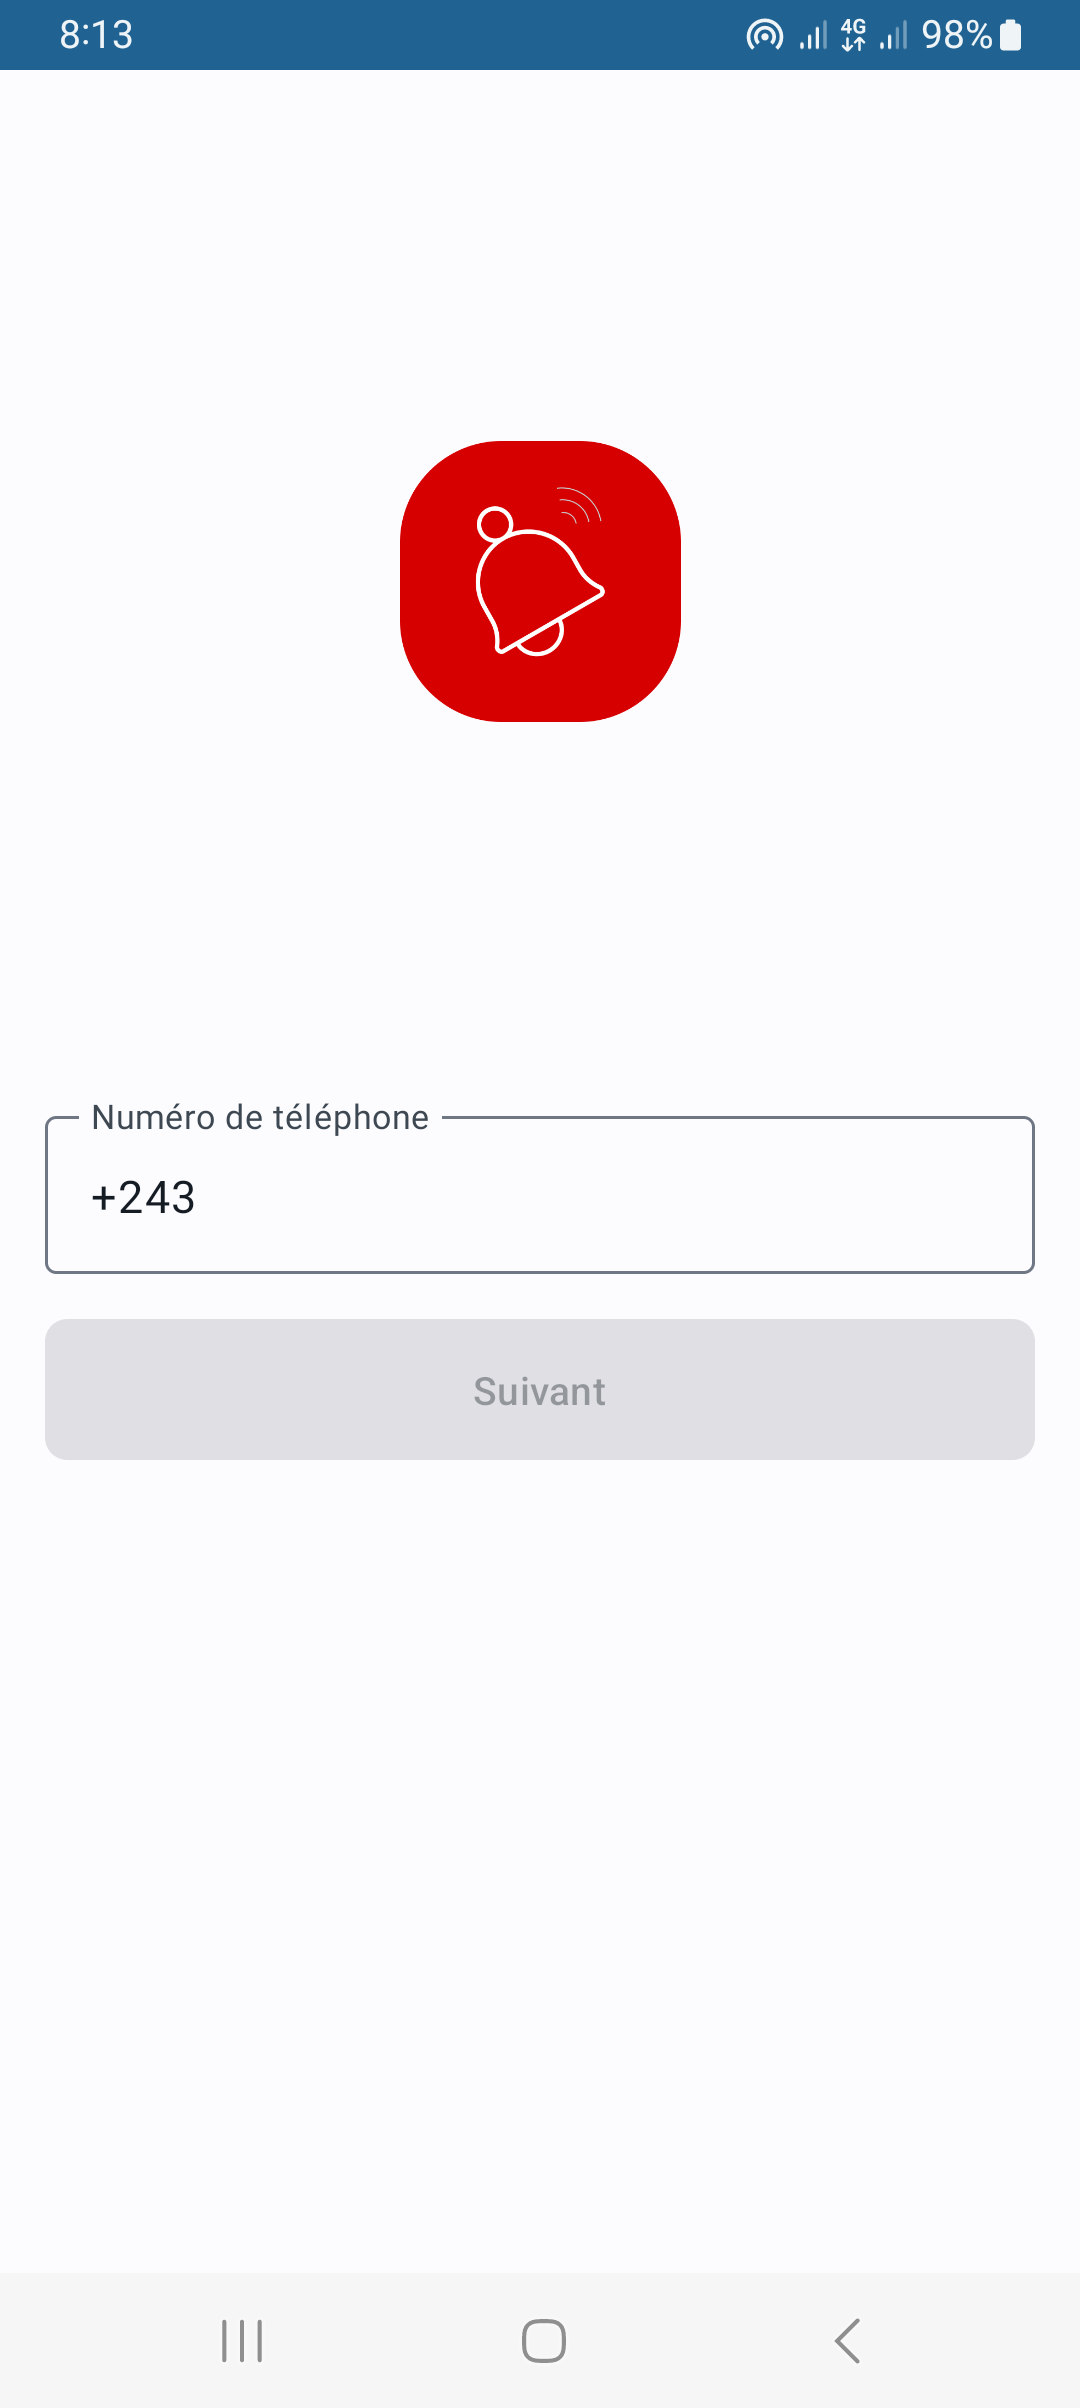
\includegraphics[width=3.6in,frame]{phone}
	\caption{Écran d’enregistrement du numéro de l’utilisateur}
\end{figure}

\begin{figure}[H]
	\centering
	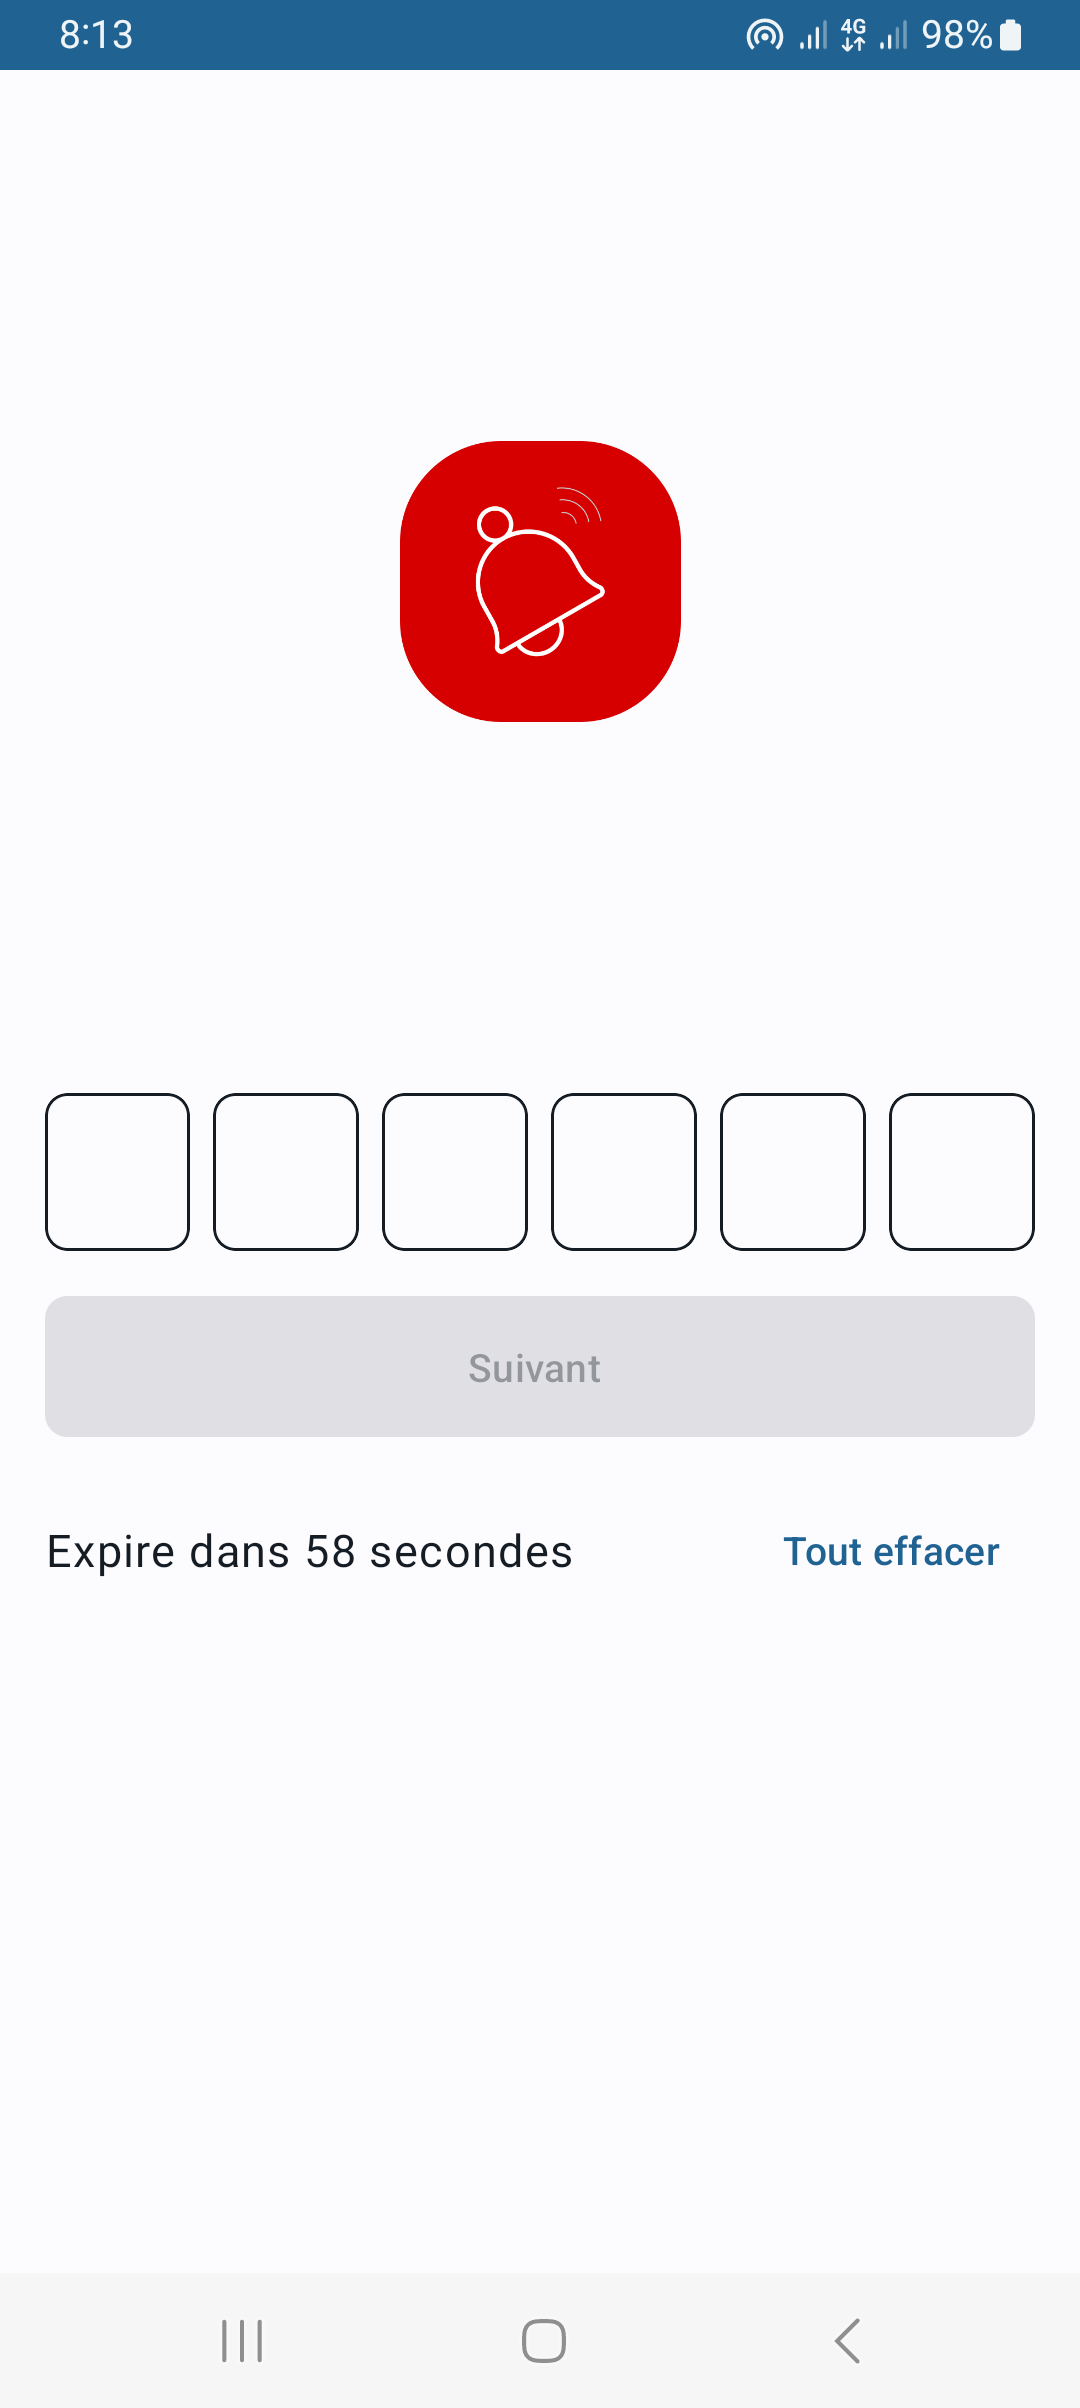
\includegraphics[width=3.6in,frame]{otp}
	\caption{Écran de soumission du code de confirmation}
\end{figure}

\begin{figure}[H]
	\centering
	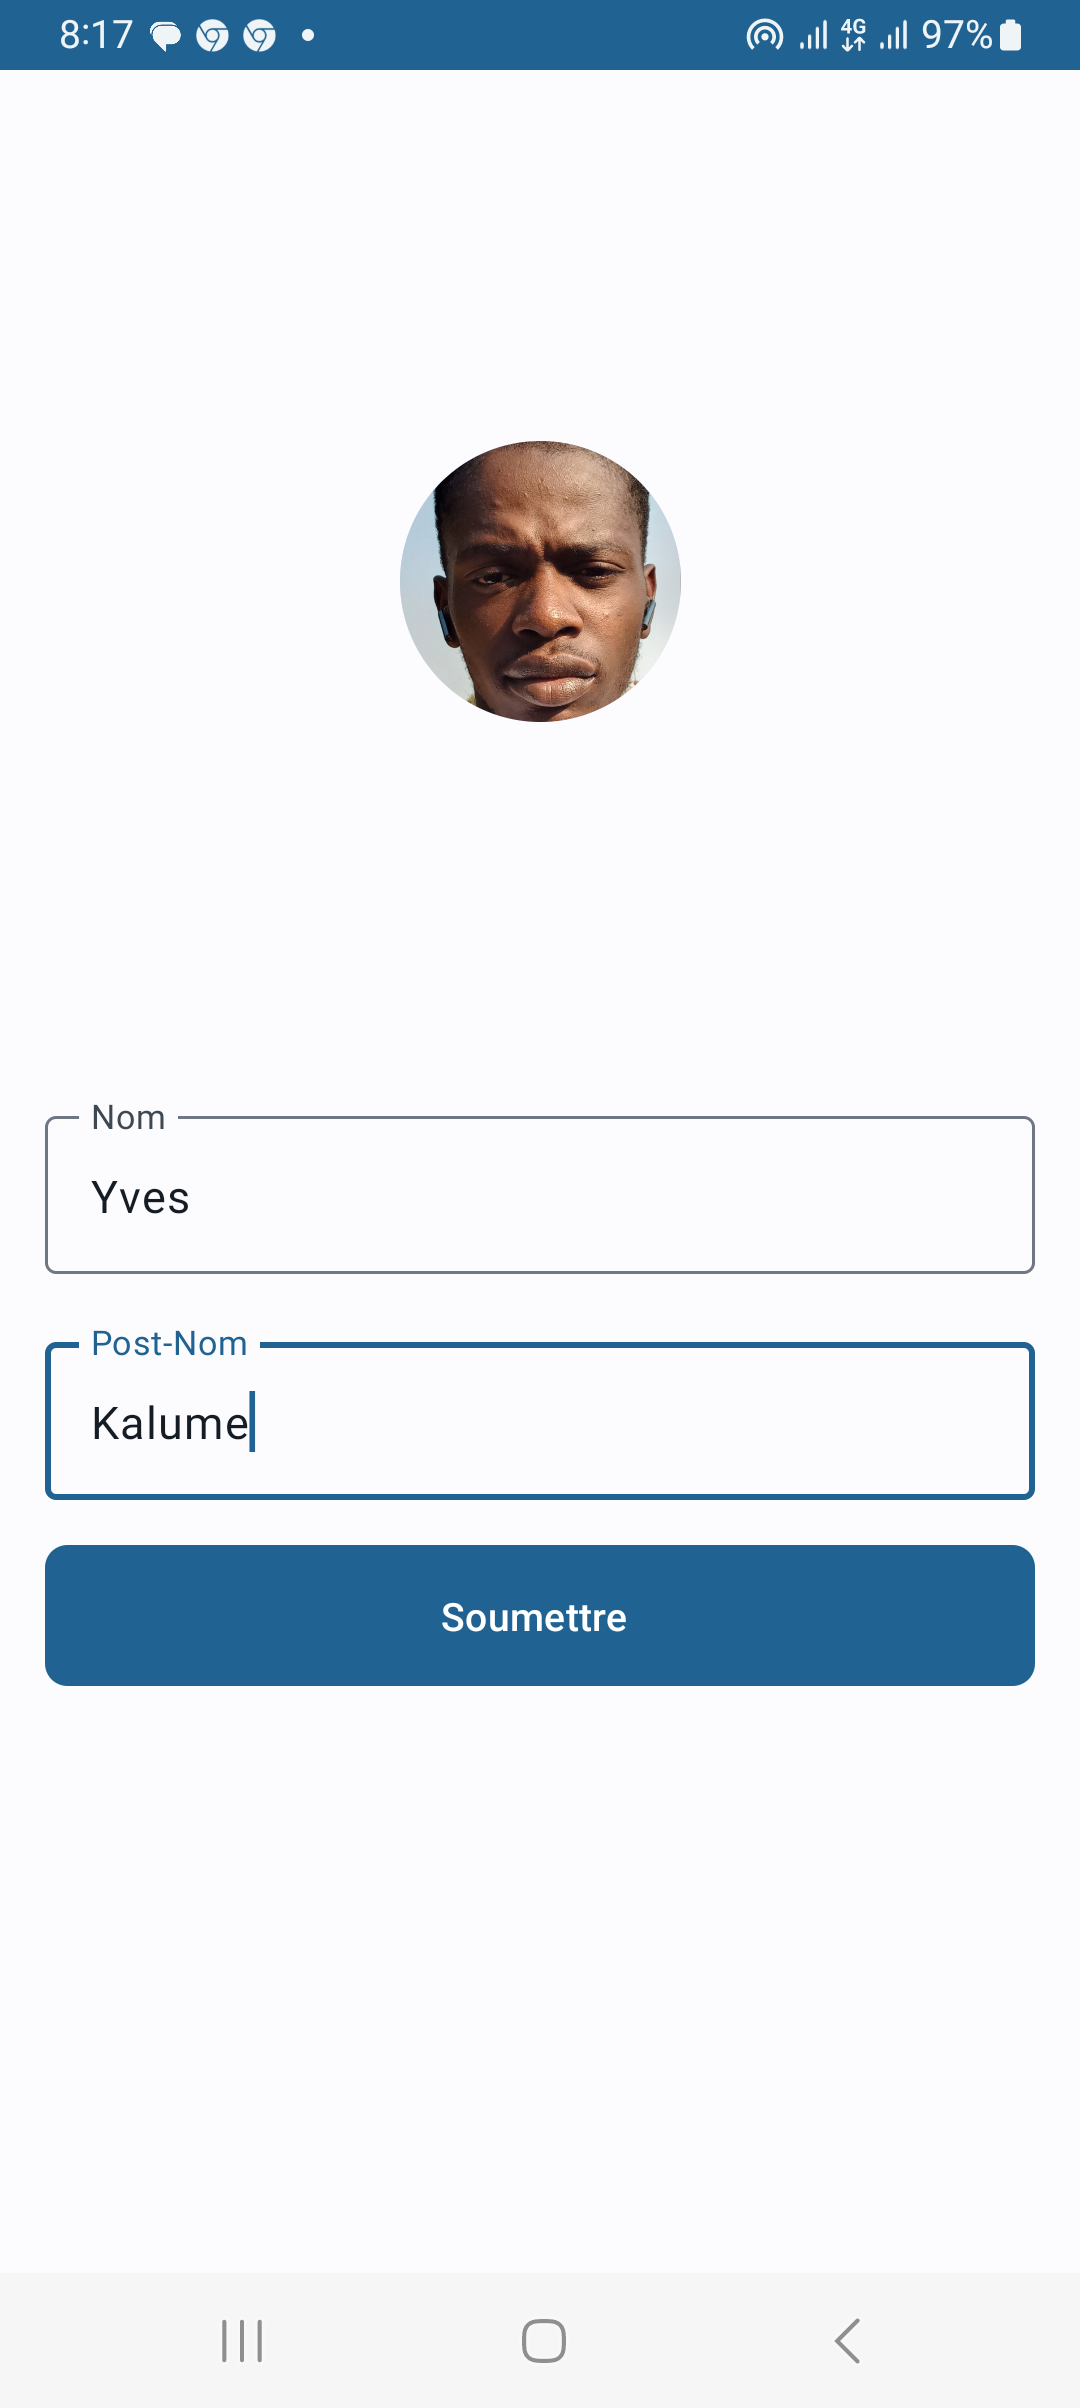
\includegraphics[width=3.6in,frame]{profile}
	\caption{Écran d’enregistrement de l’identité de l’utilisateur}
\end{figure}

\begin{figure}[H]
	\centering
	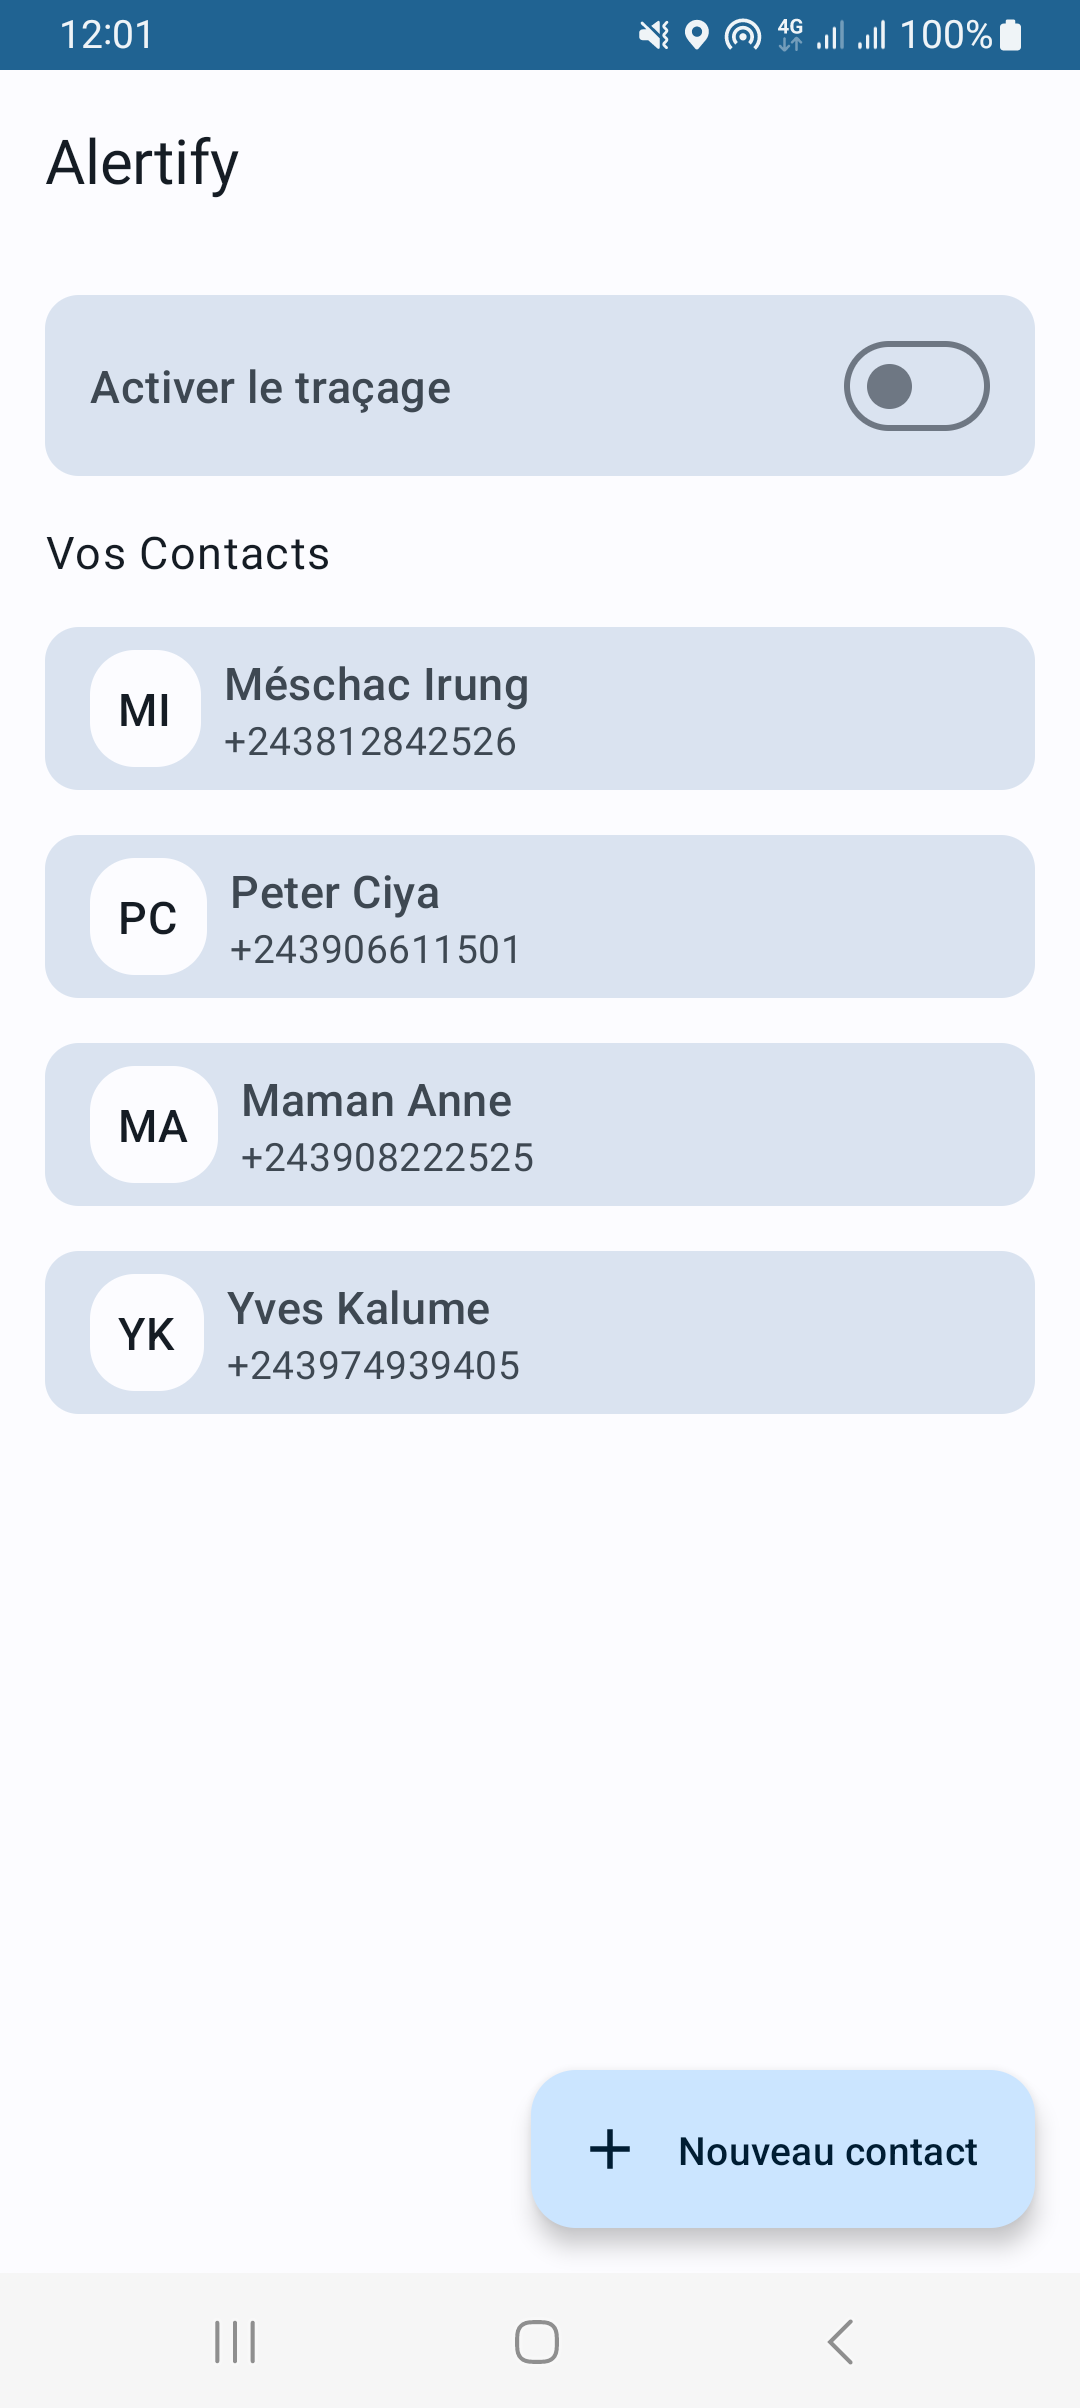
\includegraphics[width=3.6in,frame]{home}
	\caption{Écran principal}
\end{figure}

\begin{figure}[H]
	\centering
	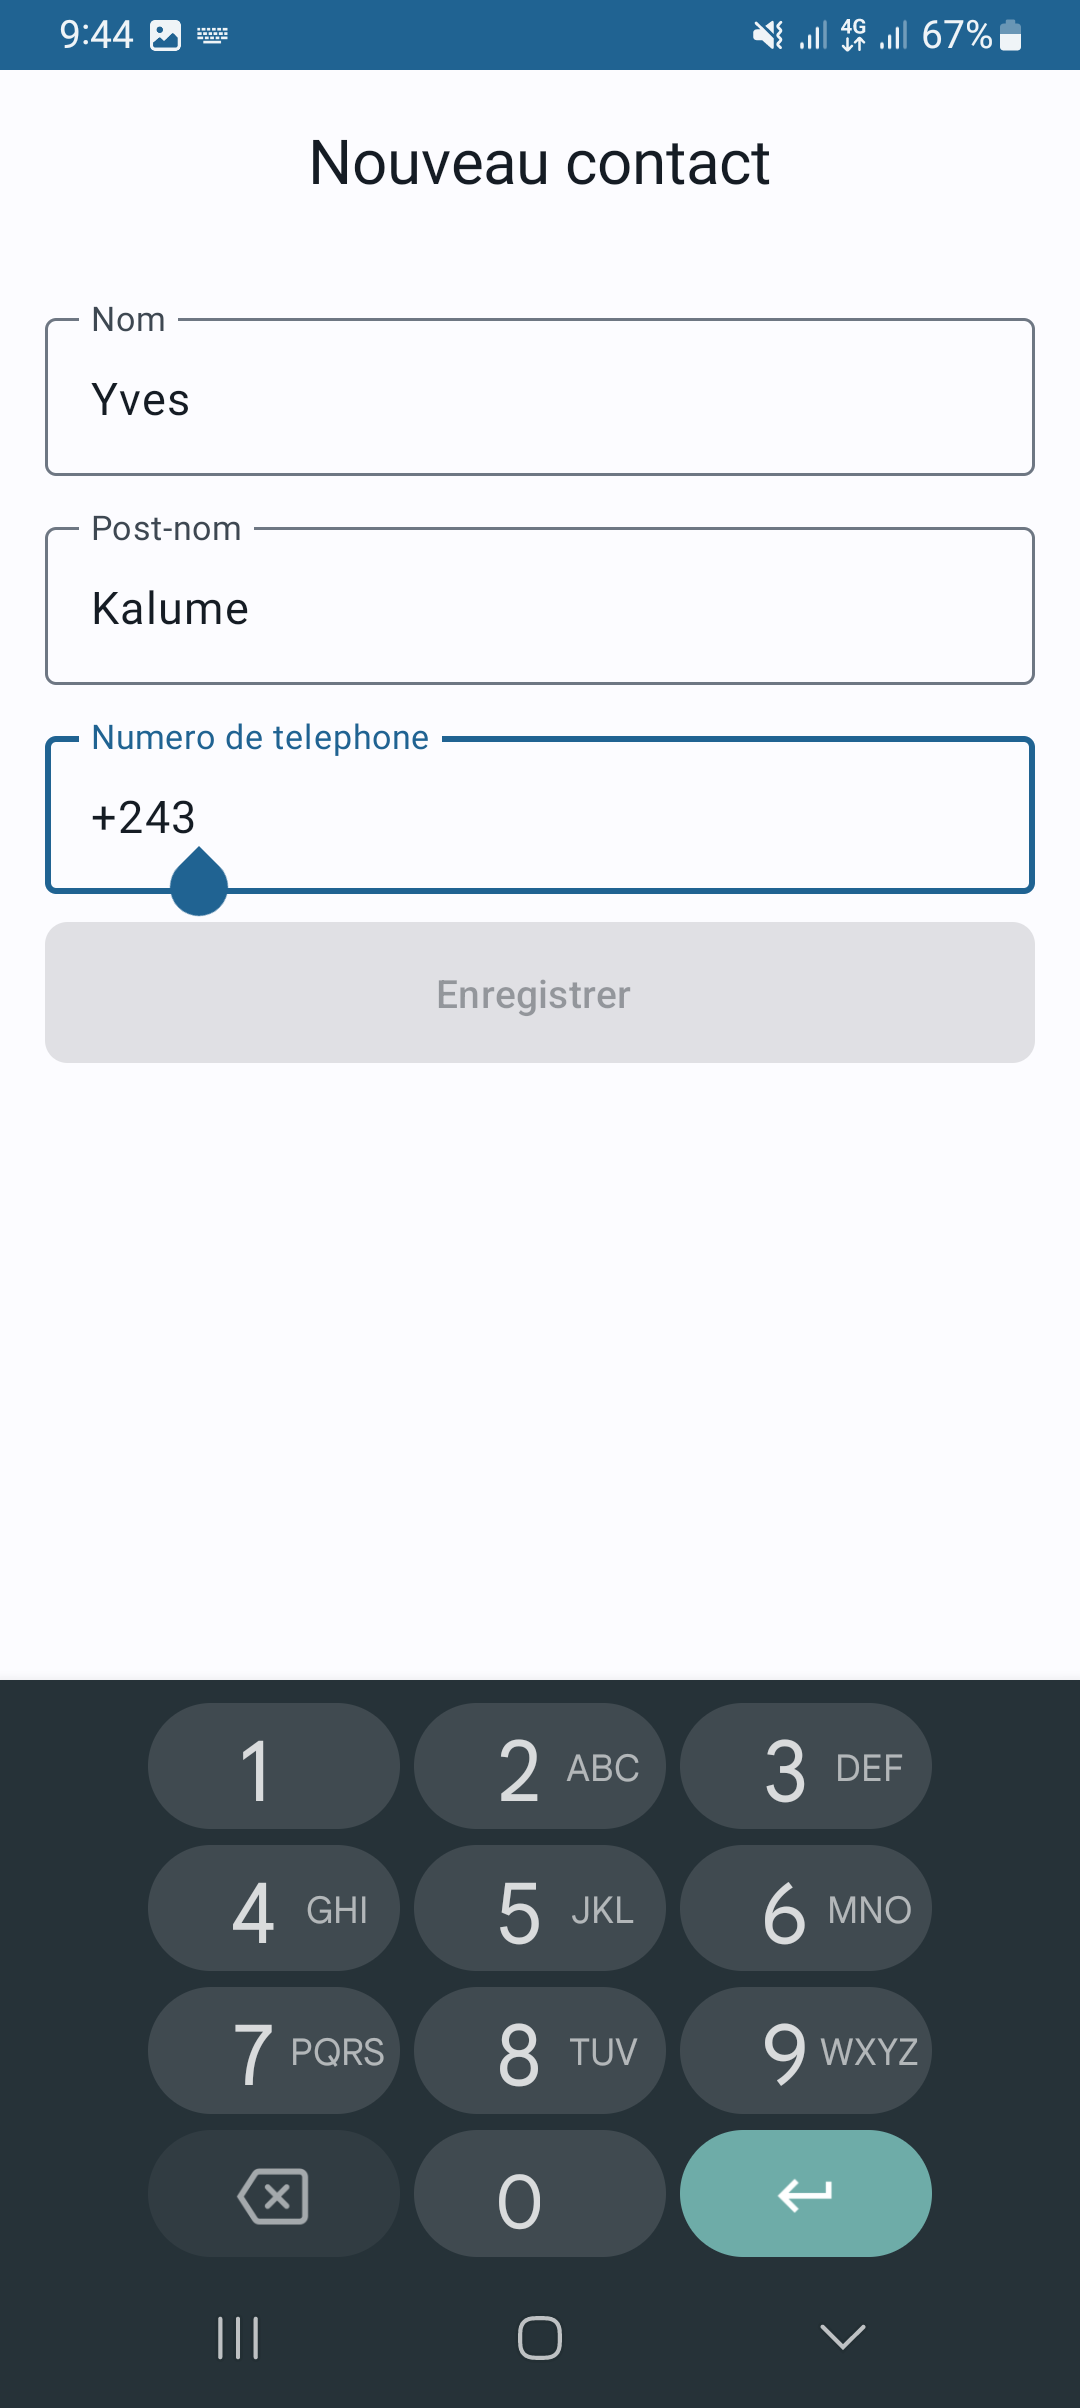
\includegraphics[width=3.6in,frame]{add_contact}
	\caption{Écran permettant d’ajouter un contact}
\end{figure}

\begin{figure}[H]
	\centering
	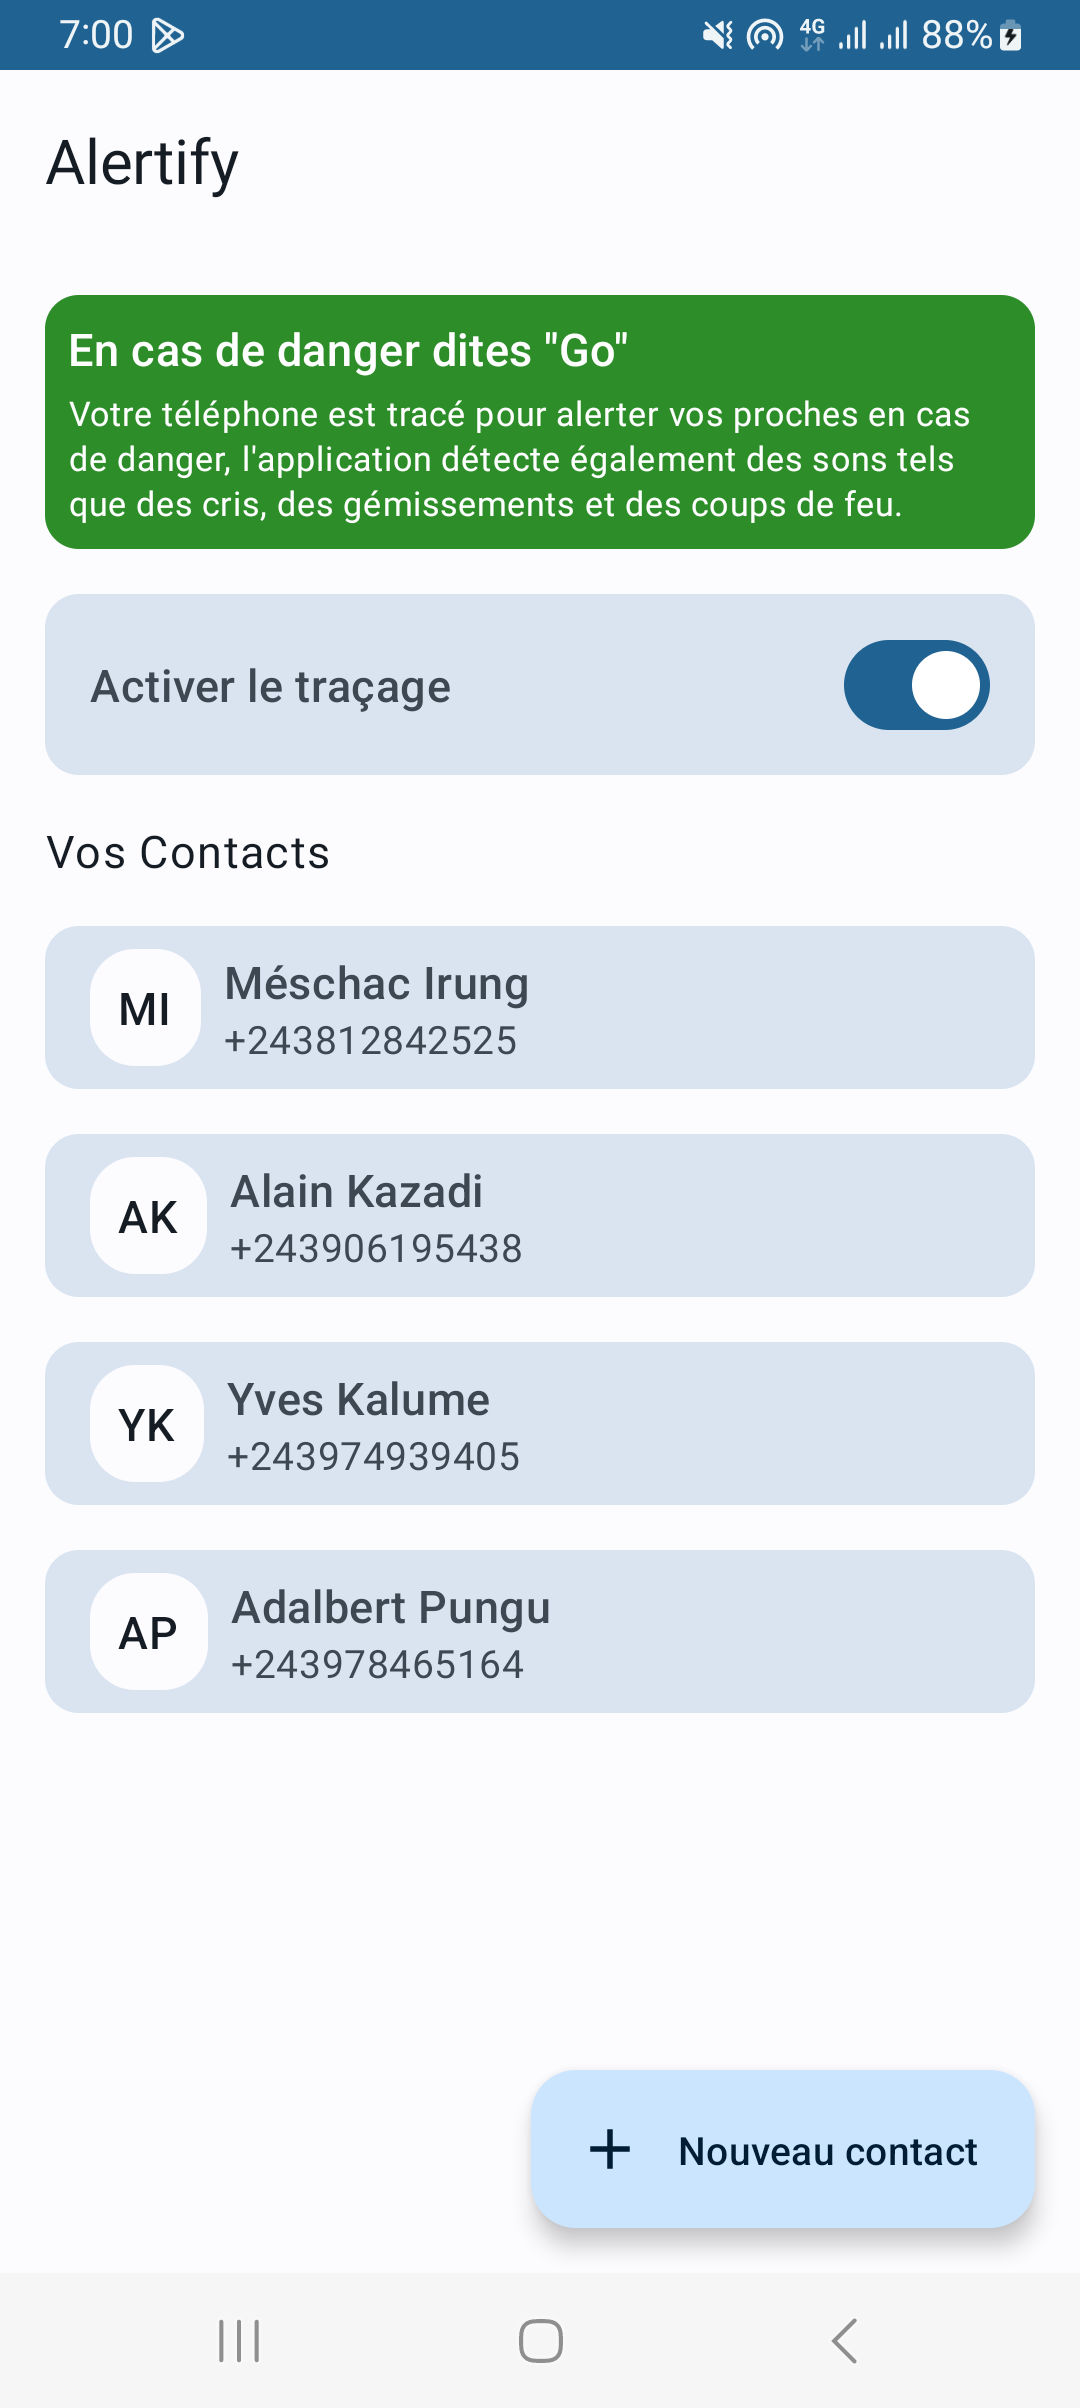
\includegraphics[width=3.6in,frame]{trackingenabled}
	\caption{Écran d'accueil, tracking activé}
\end{figure}

\begin{figure}[H]
	\centering
	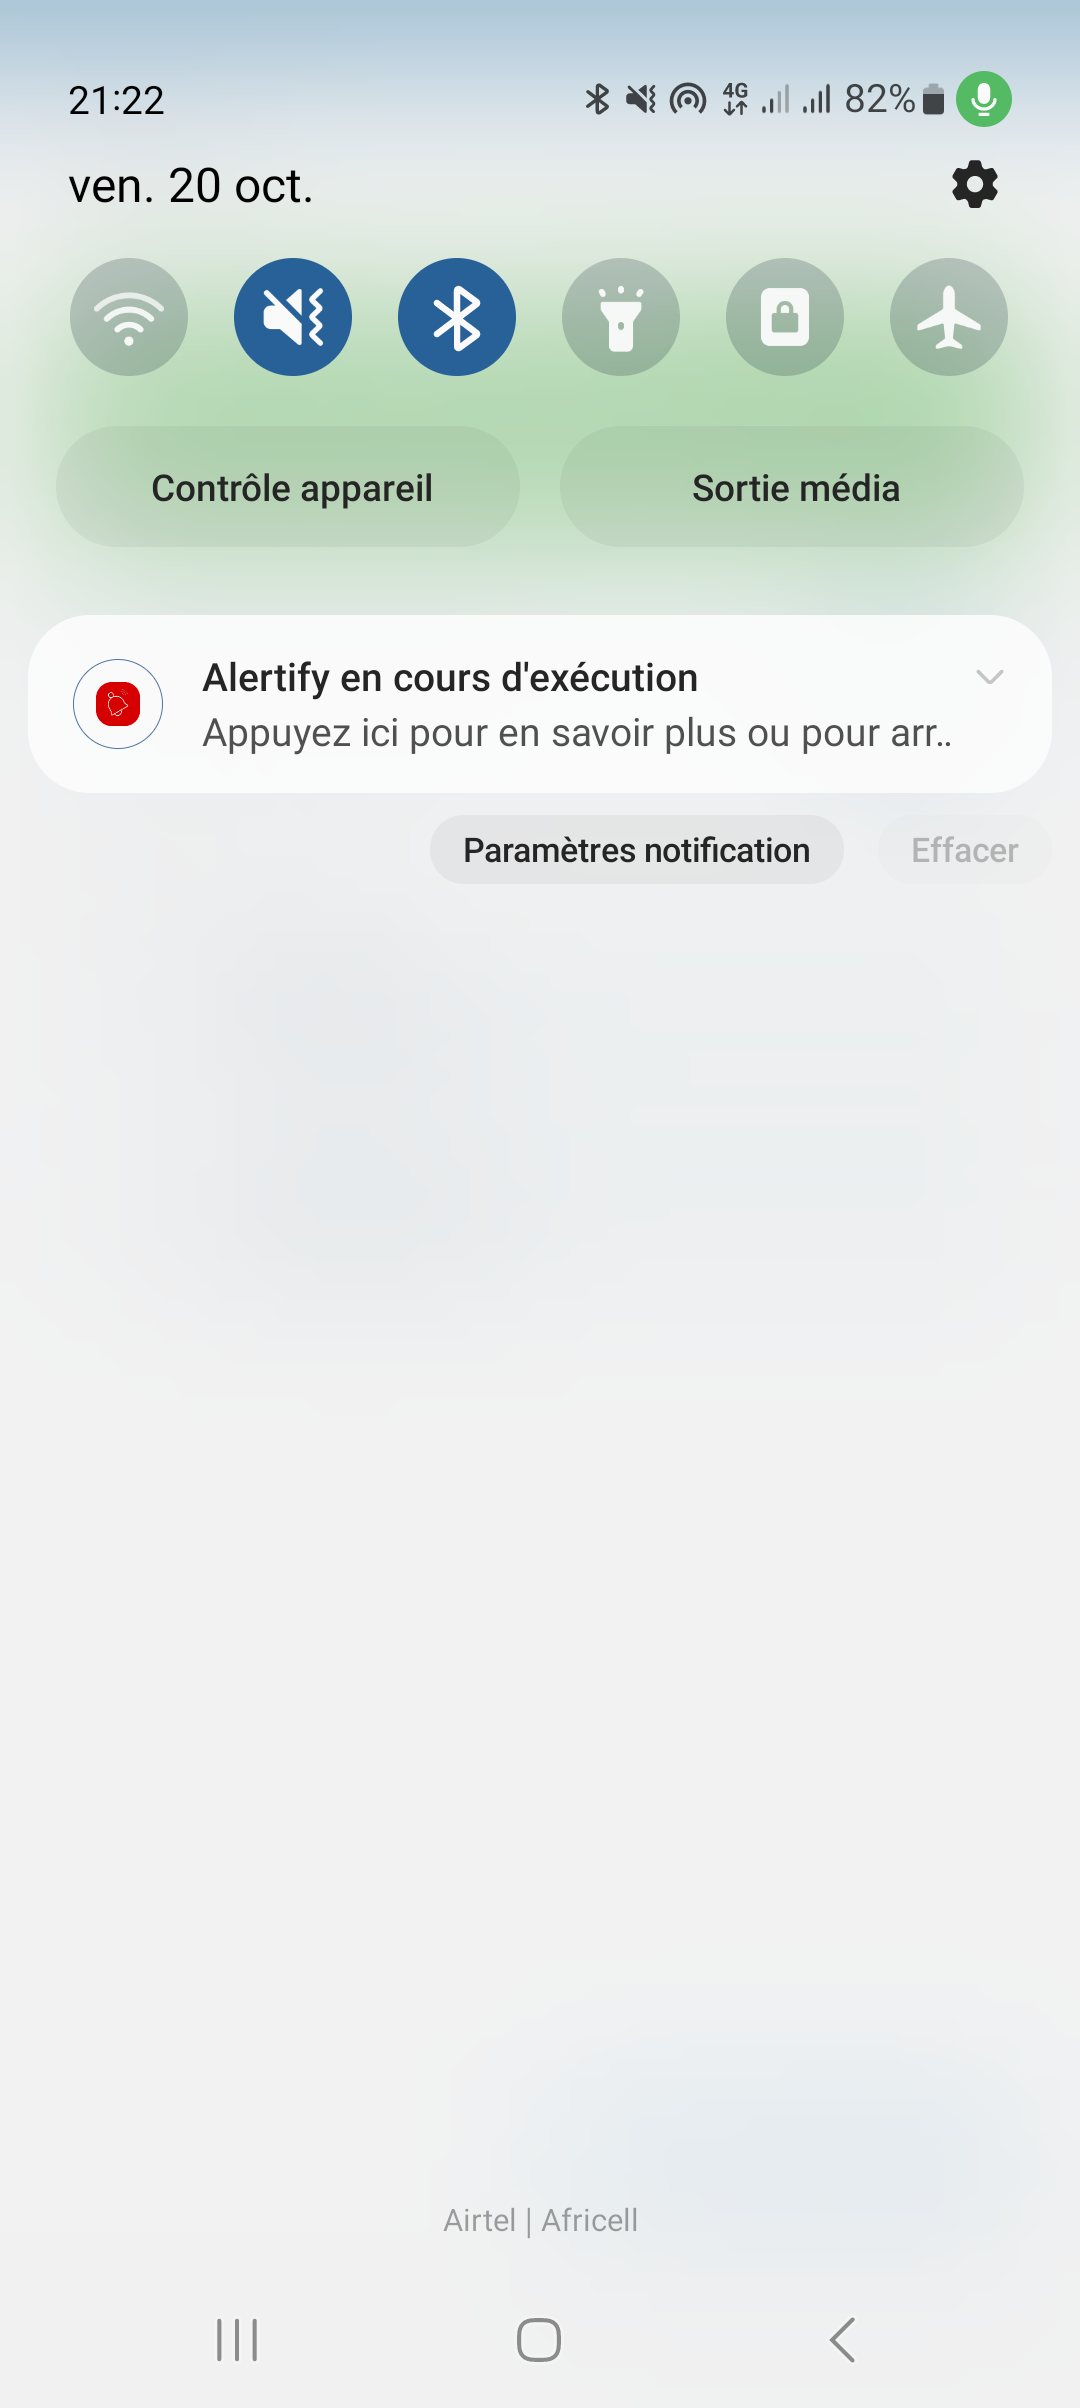
\includegraphics[width=3.6in,frame]{foreground}
	\caption{Notification signalant que le tracking est en cours}
\end{figure}

\begin{figure}[H]
	\centering
	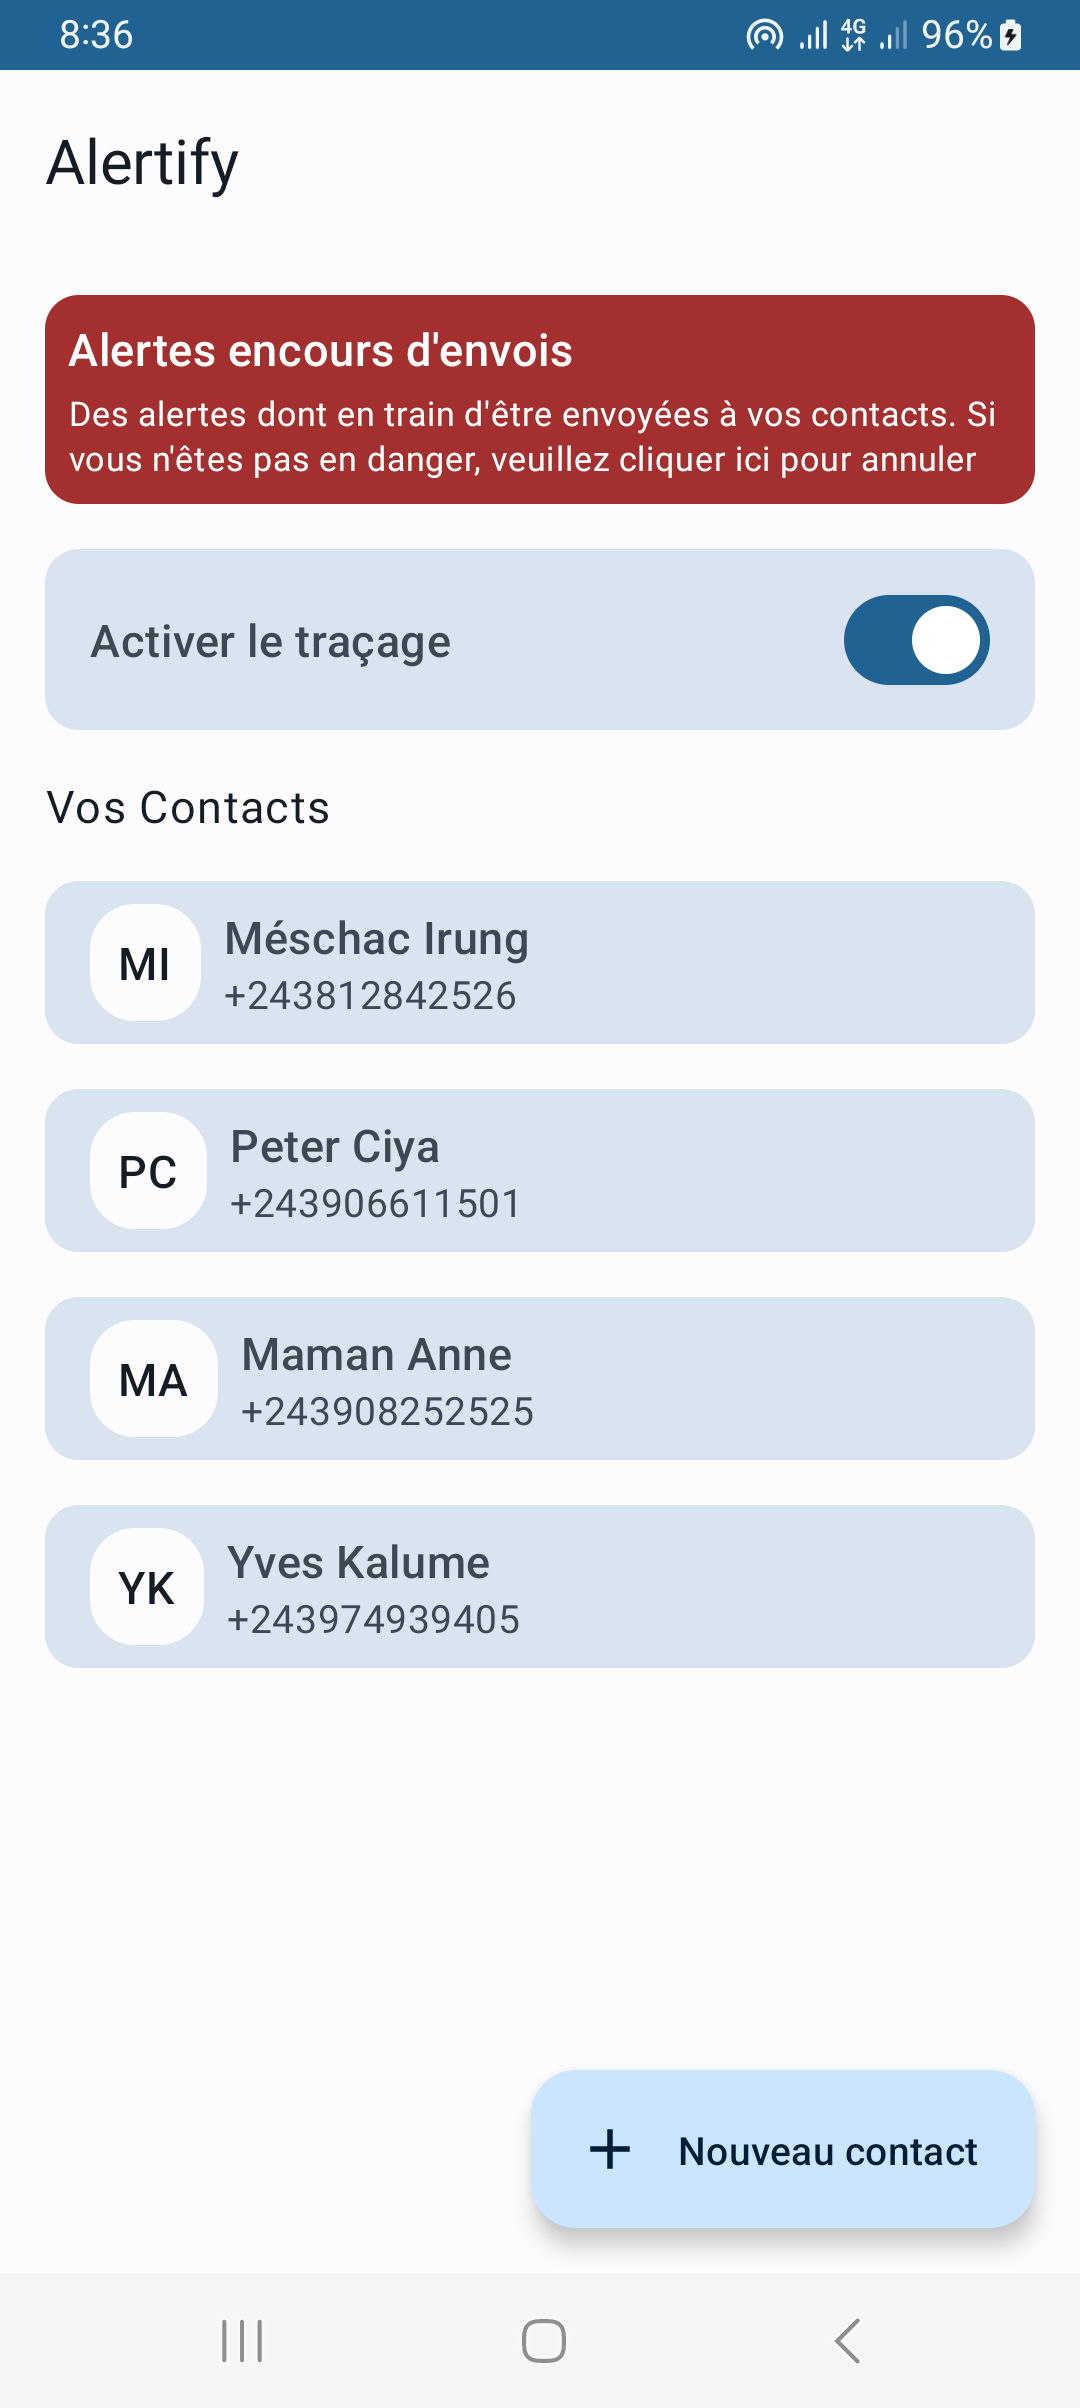
\includegraphics[width=3.6in,frame]{sendingalerts}
	\caption{Écran principal, alertes en cours d’envoi}
\end{figure}

\begin{figure}[H]
	\centering
	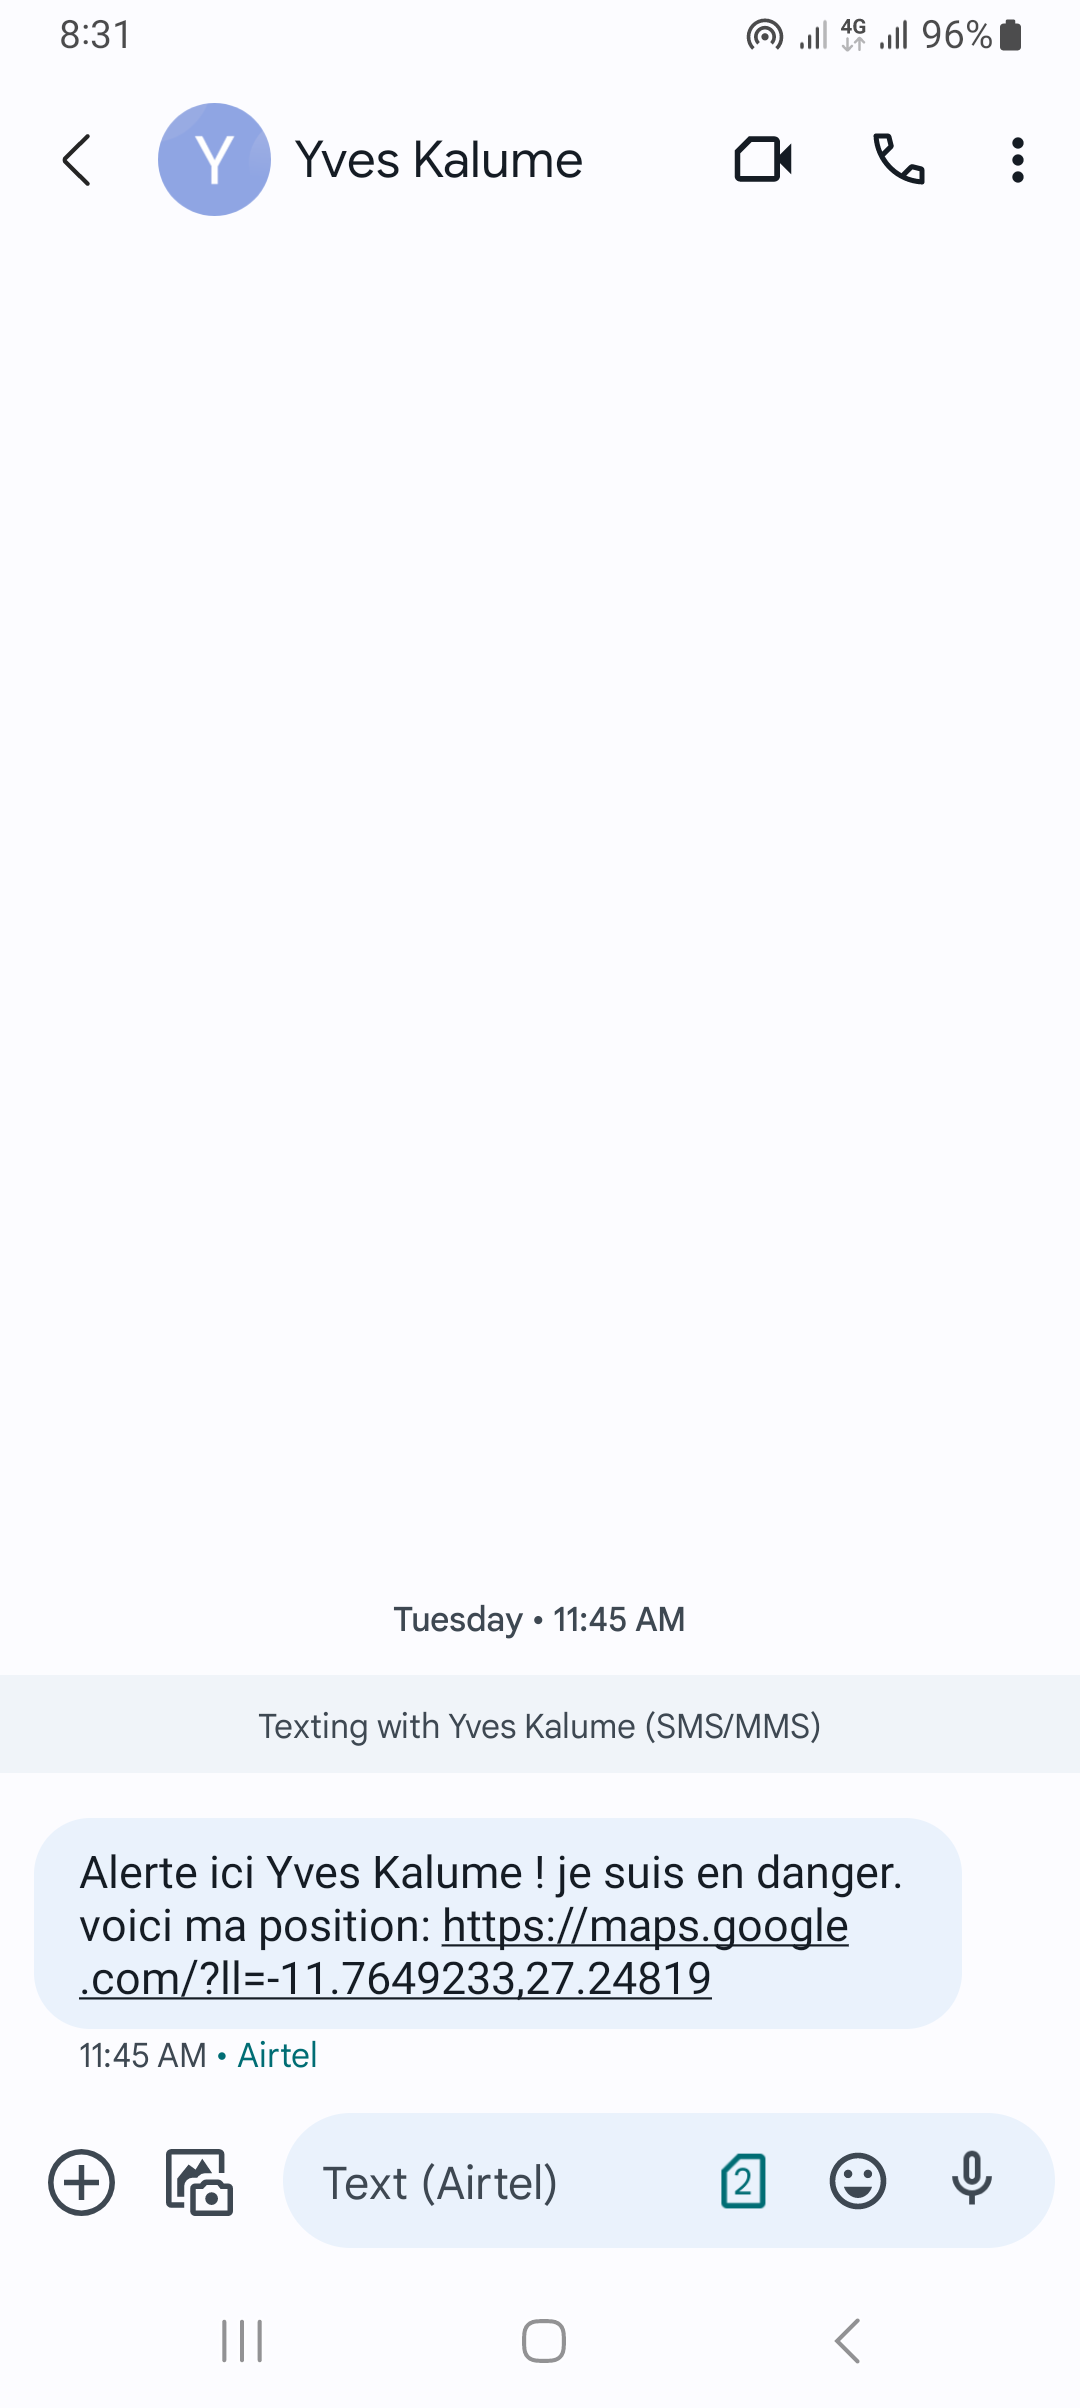
\includegraphics[width=3.6in,frame]{sms}
	\caption{SMS d’alerte}
\end{figure}

\subsection{Client web pour administrateur}

\begin{figure}[H]
	\centering
	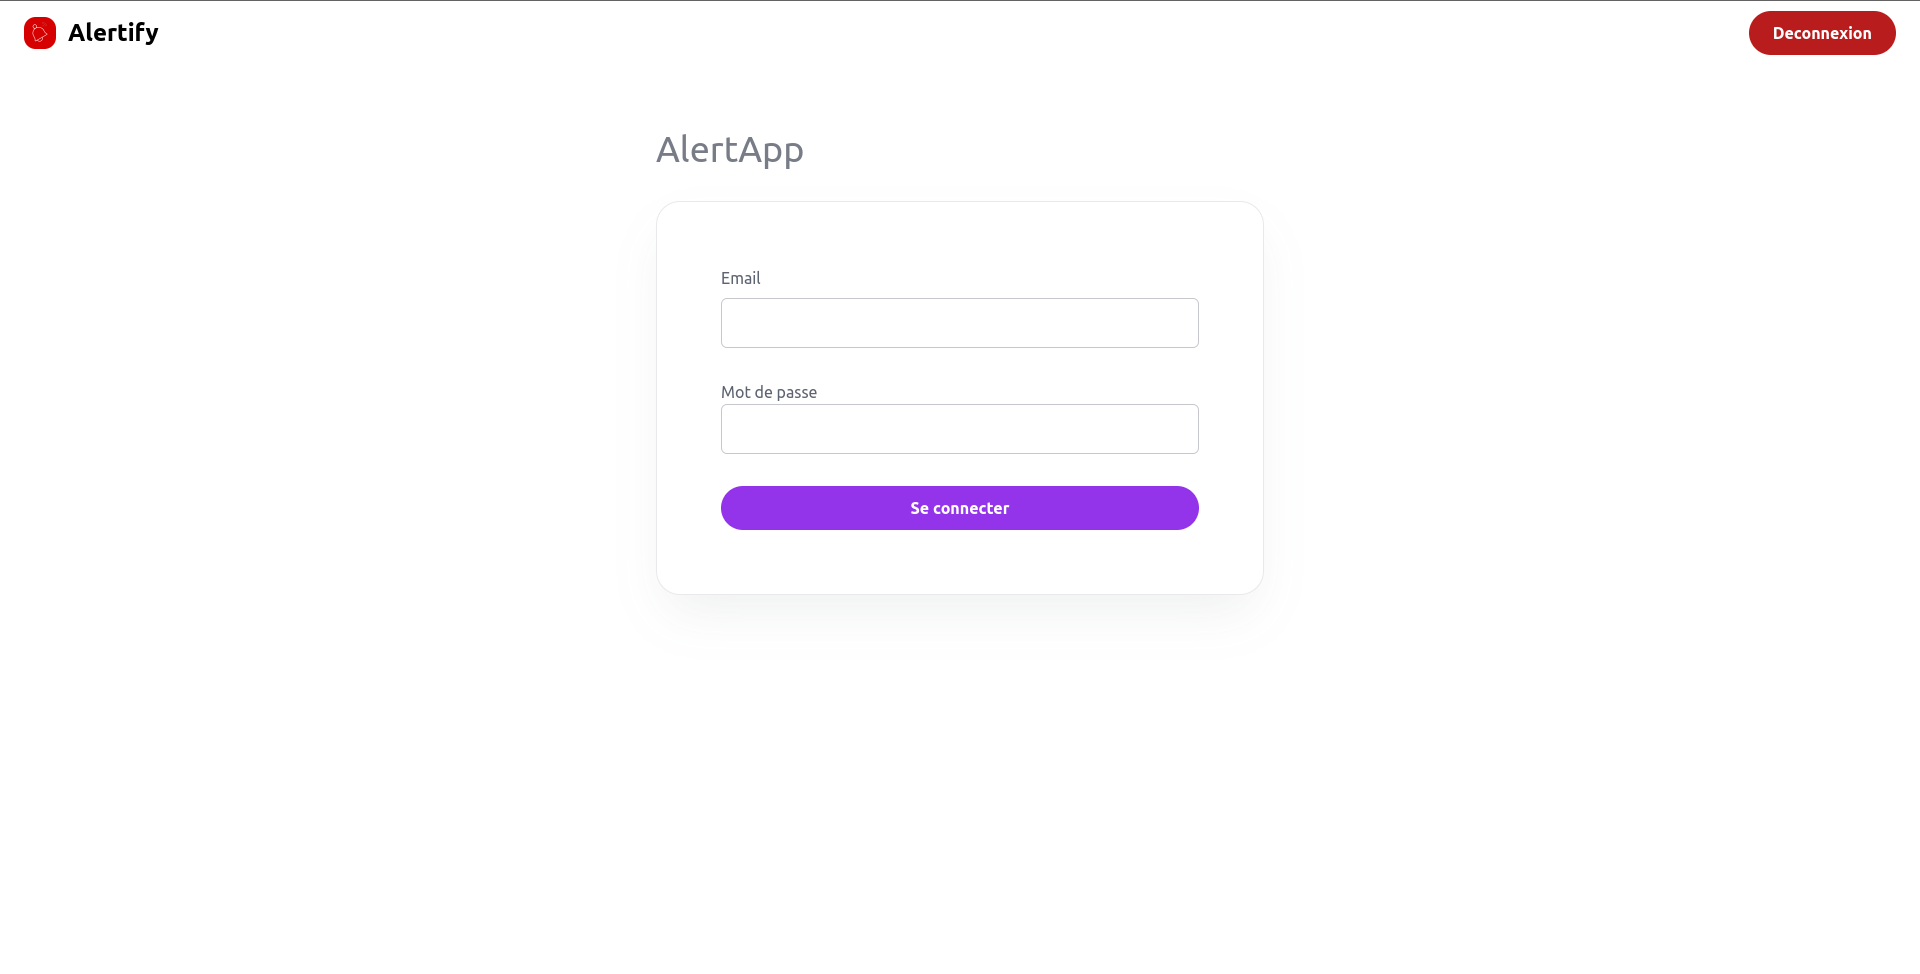
\includegraphics[width=\textwidth,frame]{admin_auth}
	\caption{Page de connexion administrateur}
\end{figure}

\begin{figure}[H]
	\centering
	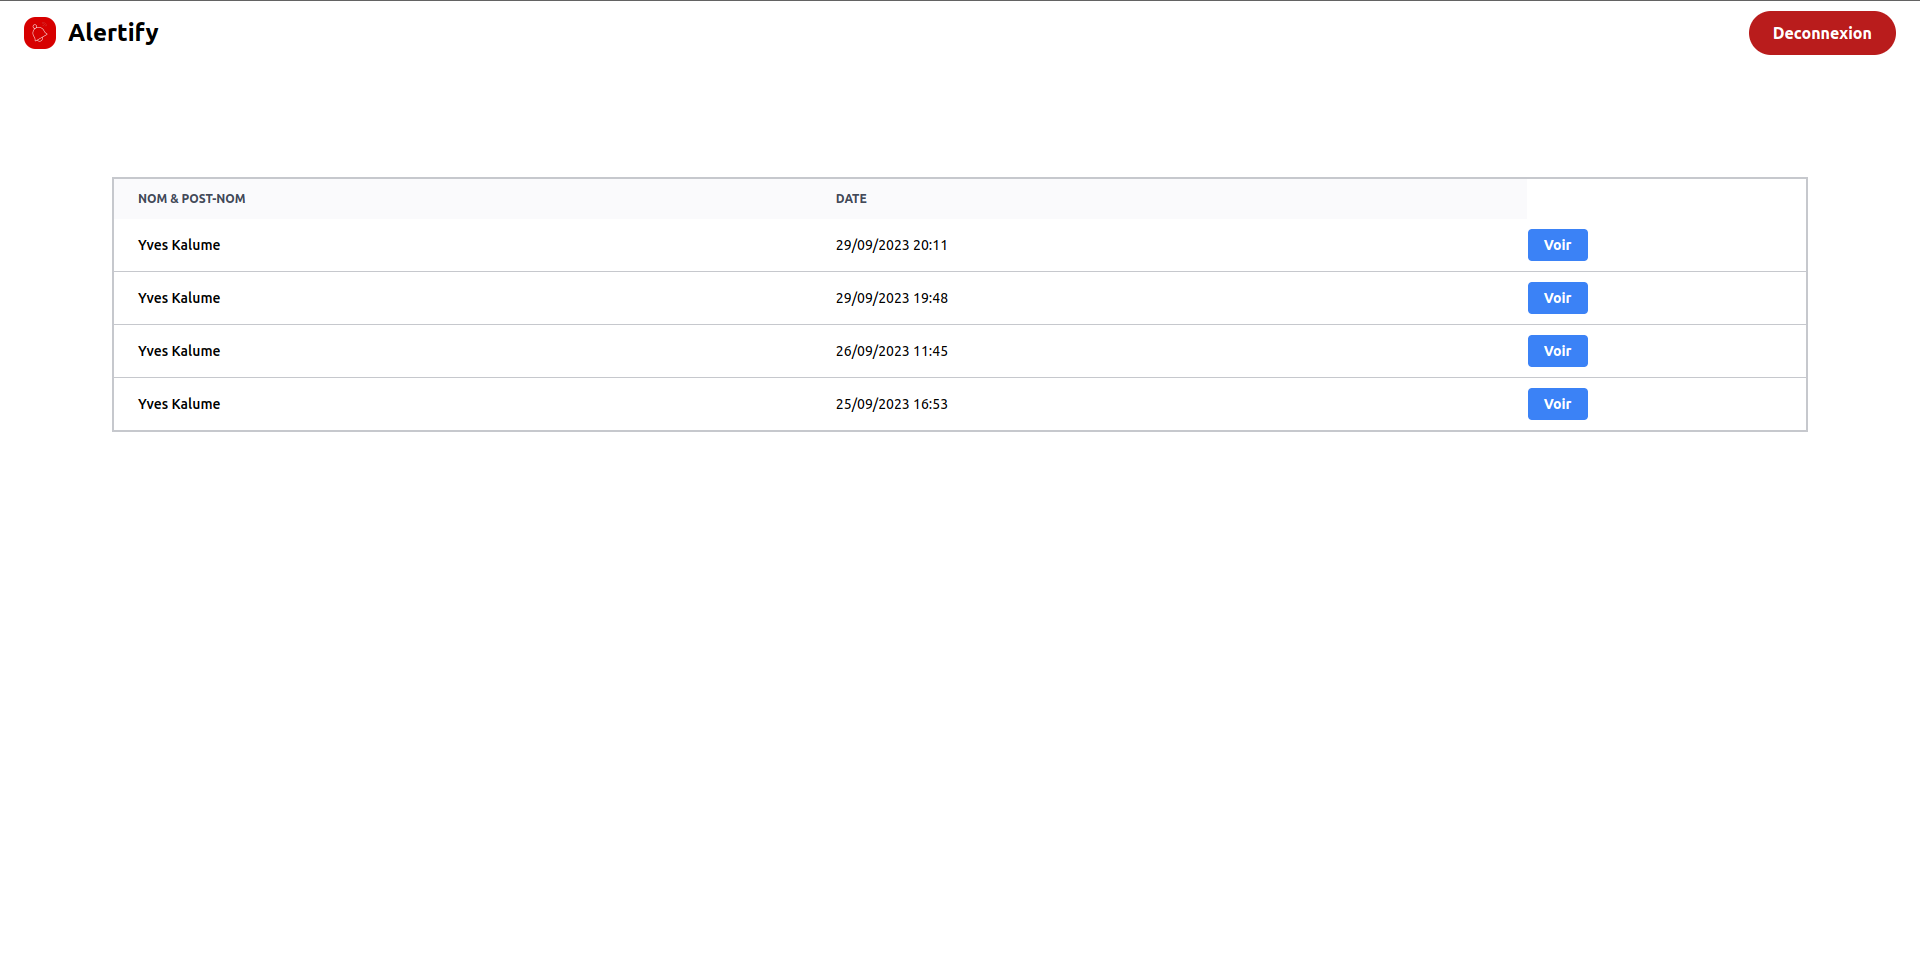
\includegraphics[width=\textwidth,frame]{admin_home}
	\caption{Listes des alertes}
\end{figure}

\begin{figure}[H]
	\centering
	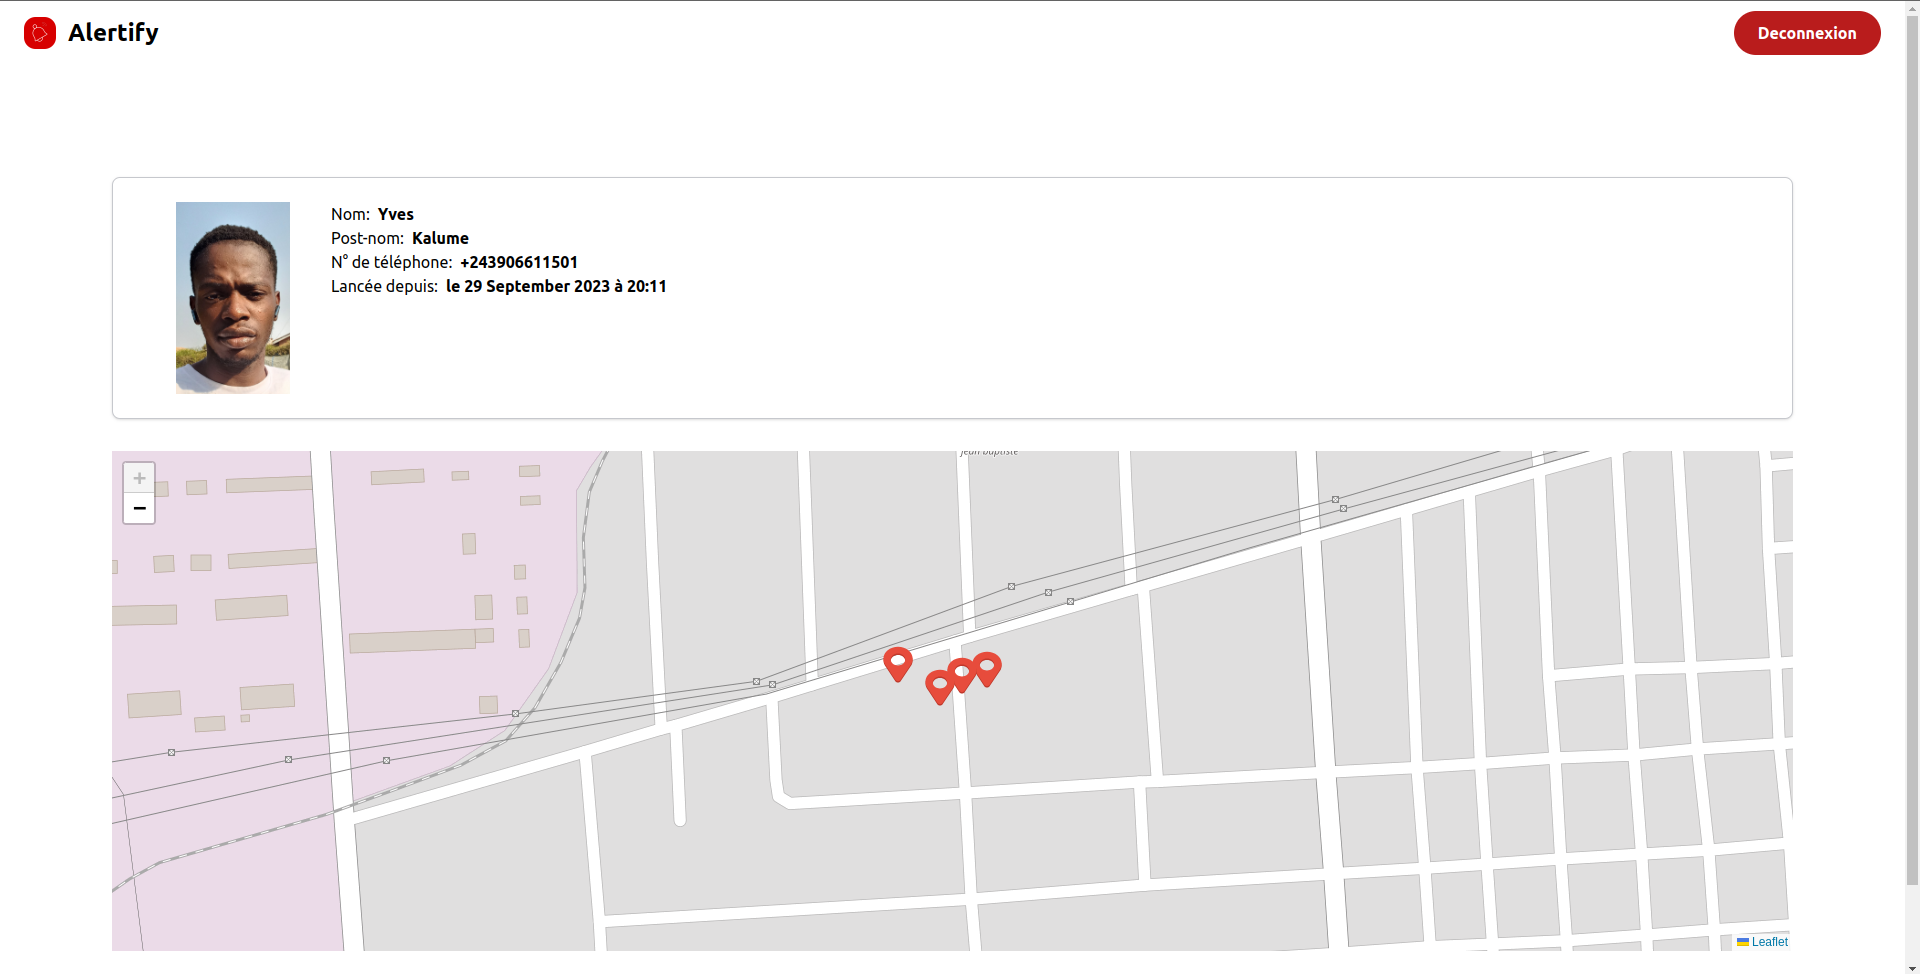
\includegraphics[width=\textwidth,frame]{admin_details}
	\caption{Détail d’une alerte}
\end{figure}

\section{Difficultés rencontrées}
Un travail scientifique vise toujours à résoudre un problème spécifique rencontré en apportant des solutions acceptables. C’est dans la recherche de cette solution que l’on oriente ses recherches dans un domaine bien déterminé et qu’on fixe les limites.

\begin{itemize}
	\item \textit{Manque d'informations des sources officielles }
\end{itemize}

Le manque d'informations fiables provenant de sources officielles a constitué un obstacle majeur. Les données sur les enlèvements, leur fréquence, leurs lieux et leurs circonstances étaient lacunaires et difficiles d'accès. Cela a compliqué notre travail d'analyse des tendances et d'adaptation de notre système aux besoins spécifiques de la ville de Lubumbashi. Nous avons dû recourir à des données disponibles, souvent limitées, et à des témoignages de la communauté locale pour informer notre approche.

\begin{itemize}
	\item \textit{Simulation de cas réels d’enlèvement}
\end{itemize}

Recréer fidèlement des cas réels d'enlèvement pour tester notre solution dans un contexte authentique s'est avéré une entreprise complexe, imprévisible et potentiellement dangereuse. La sécurité des participants est une priorité absolue, et la reproduction de situations de kidnapping authentiques implique des risques considérables. En conséquence, nous avons dû concevoir des méthodes alternatives de test qui garantissent la sécurité des participants tout en fournissant des résultats valables pour évaluer l'efficacité de notre système.\\

Ces difficultés ont mis à l'épreuve notre capacité à concevoir et à mettre en œuvre une solution efficace, tout en soulignant l'importance cruciale de l'adaptabilité et de la flexibilité pour répondre aux défis réels du terrain.

\section{ Conclusion partielle}
Ce chapitre a mis en lumière la mise en œuvre technique de notre système d'appel au secours dédié à la prévention des enlèvements dans la ville de Lubumbashi. Nous avons plongé dans les détails des algorithmes essentiels, des outils et des technologies utilisés. Au-delà des aspects techniques, nous avons également accordé une attention particulière à l'expérience utilisateur qui est un élément central pour garantir que notre solution est accessible, conviviale et efficace, enfin, nous avons parlé des défis que nous avons rencontrés et les solutions que nous avons apportées.

	\chapter*{CONCLUSION GÉNÉRALE}
\addcontentsline{toc}{chapter}{CONCLUSION GÉNÉRALE}
\justifying
Nous arrivons au terme de notre travail consacré à la conception d'un système d’appel au secours en se basant sur le cas d'enlèvement dans la ville de Lubumbashi. Nous avons parcouru un chemin jalonné de défis, d'analyses approfondies et de développements techniques pour répondre à la problématique de renforcer la sécurité et le bien-être de la communauté.\\

Nous avons avancé l'hypothèse qu'un système d'appel au secours, permettant à une victime d'enlèvement de déclencher discrètement un appel à l'aide, pourrait jouer un rôle clé dans l'amélioration de la sécurité de la ville. Pour atteindre cet objectif, nous avons exploré et développé des solutions bases sur la commande vocale et la reconnaissance sonore permettant d'alerter efficacement les contacts d'urgence et envoyer sa localisation en cas de danger imminent.\\

En fin de compte, nous espérons que notre travail contribuera à améliorer la sécurité dans la ville de Lubumbashi et à offrir aux résidents une nouvelle couche de protection en cas de danger. Cependant, nous sommes conscients que toute œuvre est teintée d'imperfections, et nous encourageons d'autres chercheurs à explorer ce même chemin pour éclaircir davantage les zones d'ombre qui subsistent.
Notre travail ne s'achève pas ici, il marque le début d'un engagement continu envers la sécurité et le bien-être de la communauté.

	\renewcommand\bibname{BIBLIOGRAPHIE}
\bibliographystyle{IEEEtran}
\bibliography{ref}
\end{document}